% ----------------------------------------------------------------
% Article Class (This is a LaTeX2e document)  ********************
% ----------------------------------------------------------------
\documentclass[12pt]{article}
\usepackage[english]{babel}
\usepackage{amsmath,amsthm}
\usepackage{amsfonts}
\usepackage{multirow}
\usepackage{color,ulem}
% THEOREMS -------------------------------------------------------
\newtheorem{thm}{Theorem}[section]
\newtheorem{cor}[thm]{Corollary}
\newtheorem{lem}[thm]{Lemma}
\newtheorem{prop}[thm]{Proposition}
\theoremstyle{definition}
\newtheorem{defn}[thm]{Definition}
\newtheorem{assum}[thm]{Assumption}
\theoremstyle{remark}
\newtheorem{rem}[thm]{Remark}
\numberwithin{equation}{section}

\usepackage{amssymb}
\newcommand{\reaction}[3]{#1 \stackrel{#3}{\leftrightharpoons} #2}
% ----------------------------------------------------------------
\begin{document}
\normalem

\title{{IMSV}: bacteria simulator specifications and architecture}%
\author{M.~Dinh}%
%\address{er}%
%\thanks{zq}%
\date{}%
% ----------------------------------------------------------------
\maketitle
\begin{abstract}
  XXX
\end{abstract}
% ----------------------------------------------------------------
\section{Introduction}

The objective of the project is to develop a simulator for a generic bacteria. The project is performed in parallel to the creation of an ontology and the associated database that describes living systems. This document presents the specifications of the simulator.


\section{Specifications}

\begin{enumerate}
  \item[F10] The simulator shall be able to simulate the following scenario:
  \begin{enumerate}
    \item different kind of (constant) extracellular conditions;
    \item upshift and downshift (change of nutritional condition) and also some stress scenarios;
    \item •	change of temperature;
    \item entry in stationary phase.
  \end{enumerate}
  \item[F20] It shall be possible to ‘kill’ a cell among others.
  \item[F30] It shall be possible to initialize the state of the simulation. (A nice to have feature: moreover some ‘aggregation’ or ‘division’ of the state may be needed for such an initialization. For instance, if a cell has been simulated with one volume, a state ‘division’ is needed to initialize a simulation with a cell simulated on several volumes.)
  \item[F40] Several stopping criterion shall be implemented:
  \begin{itemize}
    \item at the end of cellular division;
    \item simulated time exceeds a certain value;
    \item simulation time exceeds a certain value.
  \end{itemize}
      Any combination of criteria may be active.
  \item[F50] Typical values to be simulated are:
  \begin{itemize}
    \item 3e6 proteins (including proteins included in ribosomes);
    \item $[1e3 1e4]$ mRNA;
    \item $[4e3 *nb copies DNA]$  genes, each gene corresponding in mean  to  $[430 *3  basis]$;
    \item time cycle duration typically belongs to  $[20 240]$ min.
  \end{itemize}
  \item[F60] A simulation of the lifetime (cell reproduction) of a cell (Bacillus Subtilis) shall last 8 hours at most.
  \\

  \item[F70] The simulator shall output an ASCII logfile containing at least:
  \begin{itemize}
    \item the operating system;
    \item the version of the simulator and softs used;
    \item the date, the computer and the user;
    \item the localization of the data and results files.
  \end{itemize}
  \item[F80] The simulator shall be composed of 3 modules:
  \begin{itemize}
    \item the first module outputs the description of the simulation from queries of the database. This description is contained in an ASCII file that uses SBML tags to the maximum;
    \item the second module is the simulation itself. From the ASCII file provided by the first module, it outputs the simulation results in a set of ASCII files. These files shall be readable from Excel 2013 or Matlab 2012a;
    \item the third module is the analysis and visualization of the simulation results provided by the second module. (A nice to have feature is a visual representation of the simulation.)
  \end{itemize}
  \item[F90] The functionalities of the simulator shall be separated from its data and results.
  \item[F100] It shall be possible to launch a simulation interactively or by batch.
  \item[F110] It shall be possible to select the data to be recorded. By default all data shall be recorded.
  \item[F115] An option of log data / fill shall save the data necessary to restart the simulation at any given time point. Consequently, the simulator initialization has to be compatible to this data log.
  \\

  \item[F120] The cellular processes described in WholeCell shall be simulated. Beyond the simulation of a large set of cell sub-systems, a key achievement of the simulator is to be able to manage the so-called growth rate management, allowing to handle the resource balance problem. That leads to integrate in a suitable way the stringent control loop (i.e. RelA/GTP/ppGpp).
  \item[F125] xxx 1 partie moyenne (grossier) et 1 partie stochastique (fine) xxx
  \item[F130] The simulator shall be able to simulate different kind of process modeling. Typically, 4 kinds of modelling are envisaged for the process $S \ce{->} P$
  \begin{itemize}
    \item $P = f(S)$: this is a static (steady state) relation. Typically corresponding to the equilibrium manifold of a fast (and attractive) dynamics as e.g. enzymatic dynamics;
    \item $\dot{P} = f(S)$: a deterministic and continuous dynamical systems,  e.g., a detailed model of a subpart of the metabolic network (the model is deterministic but its “parameters” could be stochastics as e.g. the enzyme levels in a metabolic network);
    \item $P(nk+1) = f(P(nk),...) = P(nk)+1$: a deterministic and discrete model in time and state i.e.  the states are integer (number of). No averaging, we are at the level of one bacteria. The event (time) is assumed to be deterministic;
    \item $P(t+) = f(P(t-),...) = P(t-)+1$: a stochastic  and discrete model in time and state –see previous description.  By contrast to the previous one, the time event is assumed to be stochastics (mainly exponential distributed)
  \end{itemize}
      Furthermore, the global simulator is then  a composite set of different kinds of this modeling (among the four), however a particular sub-cellular process is modeled only by one of this modeling. \\
      Furthermore, some of the previous modeling are only possible if some “states” are available and then considered in the simulator. That is the case e.g. with respect to the metabolite concentrations.
  \item[F140] \sout{This specification assumes that it is possible to obtain metabolite pool during the simulations. The interface between the different modeling granularities is the pool of metabolites.}
  \item[F140] The set of cell-subsystems shall be defined and has to include the definition of interfaces with the the WholeCell, the possible kind of modeling (including compatibility of this modeling with the WholeCell, etc.).
  \item[F150] It shall be possible to impose the output of a particular process, typically for debug and validation (coupled with the fact that the simulation can be initialized at any time point with respect to a given  datalog of a previous simulation).
  \\

  \item[D10] The development of the simulator shall be versioned.
  \item[D20] The simulator shall be documented with:
  \begin{itemize}
    \item a user manual;
    \item a developer manual.
  \end{itemize}
  \item[D30] The simulator shall be validated on Bacillus Subtilis.
\end{enumerate}




\section{Data and states}
It is recommended to implement the simulator with the following architecture
\begin{description}
  \item Simulation object
  \begin{enumerate}
    \item Time (state)
    \item Interface between extracellular conditions (processes)
    \item Extracellular conditions 1 (object):
    \begin{enumerate}
      \item concentration of entities (glucose, metabolites, AA… or whatever) (state)
      \item evolution of the concentration (process)
    \end{enumerate}
    \item Extracellular conditions 2
    \item ...
    \item Extracellular conditions n
    \item Cell 1 (object)
    \begin{enumerate}
      \item Interface between volumes (which volume interact with which other volume and the corresponding surface) (object)
      \item Volume 1 (object)
      \begin{enumerate}
        \item Extracellular conditions (processes, numbers, surfaces) (should allow for interaction between cells through a virtual extracellular conditions)
        \item Volume (state)
        \item Number of ribosome in different states or specific ribosome and its state (Ribosome i, free occupied…) (state)
        \item Number of mRNA in different states or specific mRNA and its state (state)
        \item ...
        \item Number of metabolites in different states (state)
        \item Volume Chromosome 1: table of the same size describing the state of the chromosome (state)
        \item Volume Chromosome 2
        \item ...
        \item Volume Chromosome n (the same number as for the cell) (state)
        \item Internal (to the volume) processes
      \end{enumerate}
      \item Volume 2
      \item ...
      \item Volume n
      \item Cell Chromosome 1 (object):
      \begin{enumerate}
        \item Table of ‘mère’ / ‘filles’ (state)
        \item Table (size = number of structure (gene or codon or groups of codons) x maximal number of ‘brindilles’) with the number of the cell containing the structure. By convention, 0 = non active/does not exist; -1 = to fork (go the chromosomes ‘filles’); -2 = from fork (go the chromosome ‘mère’) (state)
        \item Description of the structures (which AA needed), description of the genes (which structures, to produce what) (data)
      \end{enumerate}
      \item Cell Chromosome 2 if needed
      \item ...
      \item Cell Chromosome n if needed
      \item Internal (to the cell) processes, typically replication or DNA movement from a volume to another one
      \end{enumerate}
    \item Cell 2
    \item ...
    \item Cell n
  \end{enumerate}
\end{description}
Basically, cell only communicate with extracellular conditions. Each cell is divided into volumes that can communicate either with extracellular conditions or other volumes of the same cell. The chromosome is divided into 'cell chromosome' which handles the continuity of the chromosome and 'volume chromosome' which handles transcription and translation.



\subsection{Chromosome}
There are 'cell chromosome' and 'volume chromosome' because we wish that only a higher level object may access to the data and state of a lower object; this distinction is otherwise not needed and the chromosome object should be placed at cell level. 'Cell chromosome' mainly handles the continuity of the chromosome of the cell through all the volumes. 'Volume chromosome' directly handles the biological process internally to each volume. 'Cell chromosome' and 'volume chromosome' must be coherent.


\paragraph{Representation} A chromosome is represented in a condensed way in the simulator. In fact depending on the aggregation performed, the representation can be more or less fine.
\begin{center}
\begin{tabular}{|c|c|}
  \hline
  % after \\: \hline or \cline{col1-col2} \cline{col3-col4} ...
  NTP 1  & \multirow{1}{*}{NTP aggregation 1} \\
  \hline
  NTP 2  & \multirow{3}{*}{NTP aggregation 2} \\
  NTP 3  &  \\
  NTP 4  &  \\
  \hline
  NTP 5  & \multirow{5}{*}{NTP aggregation 3} \\
  NTP 6  &  \\
  NTP 7  &  \\
  NTP 8  &  \\
  NTP 9  &  \\
  \hline
  NTP 10 & \multirow{2}{*}{NTP aggregation 4} \\
  NTP 11 &  \\
  \hline
  NTP 12 & \multirow{10}{*}{NTP aggregation 5} \\
  NTP 13 &  \\
  NTP 14 &  \\
  NTP 15 &  \\
  NTP 16 &  \\
  NTP 17 &  \\
  NTP 18 &  \\
  NTP 19 &  \\
  NTP 20 &  \\
  NTP 21 &  \\
  \hline
  NTP 22 & \multirow{9}{*}{NTP aggregation 6} \\
  NTP 23 &  \\
  NTP 24 &  \\
  NTP 25 &  \\
  NTP 26 &  \\
  NTP 27 &  \\
  NTP 28 &  \\
  NTP 29 &  \\
  \hline
  NTP 30 & \multirow{1}{*}{NTP aggregation 7} \\
  \hline
\end{tabular}
\end{center}
Note that with this aggregation, there are some conflicts between DNA replication / transcription and DNA damage / repair / mutation... Unless some rules are enforced to solve the conflicts, it is not possible to have different kind of process be performed the same time on a NTP aggregation.
\begin{assum}
\begin{enumerate}
  \item To avoid change of a volume state to another one due to, for instance, a polymerase changing of volume, it is assumed that a gene is necessary contained in one volume;
  \item The decomposition into NTP aggregations applies to any biological process related to DNA (replication, transcription, translation and manipulation).
\end{enumerate}
\end{assum}
\noindent This assumption should not too drastic as a gene is much smaller than a chromosome.


\subsubsection{Cell Chromosome}
\paragraph{Evolution state} For DNA replication purpose, it is needed to represent fork. It is assumed that the maximal number of forks $n$ in known and that the considered chromosome is represented by $m$ NTP aggregations. Then, the chromosome can be represented by 3 tables:
\begin{enumerate}
  \item a main table of size $m \times \sum_{i=0}^n2^i$ containing the number of the volume where it is. Moreover, -1 means go to 'mother', -2 means go to 'daughters' and -3 means go both to 'mother' and 'daughters';
  \item a 'mother' table of size $1 \times \sum_{i=0}^n2^i$ representing one strand of the fork;
  \item a 'daughters' table of size $2 \times \sum_{i=0}^n2^i$ representing the two last strands of the fork.
\end{enumerate}

\medskip

We now illustrate how it works. Assume that the chromosome (with $n=2$ and $m=10$) does not have any fork yet and is contained in the volume 2, then the tables are
\begin{center}
  \begin{tabular}{|c|r|r|r|r|r|r|r|}
     \hline
     % after \\: \hline or \cline{col1-col2} \cline{col3-col4} ...
     \multirow{10}{*}{Main table} & 2 & 0 & 0 & 0 & 0 & 0 & 0 \\
     & 2 & 0 & 0 & 0 & 0 & 0 & 0 \\
     & 2 & 0 & 0 & 0 & 0 & 0 & 0 \\
     & 2 & 0 & 0 & 0 & 0 & 0 & 0 \\
     & 2 & 0 & 0 & 0 & 0 & 0 & 0 \\
     & 2 & 0 & 0 & 0 & 0 & 0 & 0 \\
     & 2 & 0 & 0 & 0 & 0 & 0 & 0 \\
     & 2 & 0 & 0 & 0 & 0 & 0 & 0 \\
     & 2 & 0 & 0 & 0 & 0 & 0 & 0 \\
     & 2 & 0 & 0 & 0 & 0 & 0 & 0 \\
     \hline \hline
     'Mother' table & 0 & 0 & 0 & 0 & 0 & 0 & 0 \\
     \hline \hline
     \multirow{2}{*}{'Daughters' table} & 0 & 0 & 0 & 0 & 0 & 0 & 0 \\
     & 0 & 0 & 0 & 0 & 0 & 0 & 0 \\
     \hline
   \end{tabular}
\end{center}
Now assume that the NTP aggregation 1 to 5 and 7 to 10 were replicated, one strand being in the volume 2 and the other one in the volume 1, the tables are
\begin{center}
  \begin{tabular}{|c|r|r|r|r|r|r|r|}
     \hline
     % after \\: \hline or \cline{col1-col2} \cline{col3-col4} ...
     \multirow{10}{*}{Main table} & 0 &  2 &  1 & 0 & 0 & 0 & 0 \\
     &  0 &  2 &  1 & 0 & 0 & 0 & 0 \\
     &  0 &  2 &  1 & 0 & 0 & 0 & 0 \\
     &  0 &  2 &  1 & 0 & 0 & 0 & 0 \\
     & -2 &  2 &  1 & 0 & 0 & 0 & 0 \\
     &  2 & -1 & -1 & 0 & 0 & 0 & 0 \\
     & -2 &  2 &  1 & 0 & 0 & 0 & 0 \\
     &  0 &  2 &  1 & 0 & 0 & 0 & 0 \\
     &  0 &  2 &  1 & 0 & 0 & 0 & 0 \\
     &  0 &  2 &  1 & 0 & 0 & 0 & 0 \\
     \hline \hline
     'Mother' table & 0 & 1 & 1 & 0 & 0 & 0 & 0 \\
     \hline \hline
     \multirow{2}{*}{'Daughters' table} & 2 & 0 & 0 & 0 & 0 & 0 & 0 \\
     & 3 & 0 & 0 & 0 & 0 & 0 & 0 \\
     \hline
   \end{tabular}
\end{center}
Assume that there is another fork in the volume 1 for the NTP aggregation 1 only contained in volume 1 also while a part of the strand moved to volume 3, then the tables are
\begin{center}
  \begin{tabular}{|c|r|r|r|r|r|r|r|}
     \hline
     % after \\: \hline or \cline{col1-col2} \cline{col3-col4} ...
     \multirow{10}{*}{Main table} & 0 &  2 & -2 &  1 &  1 & 0 & 0 \\
     &  0 &  2 &  1 & -1 & -1 & 0 & 0 \\
     &  0 &  2 &  1 &  0 &  0 & 0 & 0 \\
     &  0 &  2 &  1 &  0 &  0 & 0 & 0 \\
     & -2 &  2 &  1 &  0 &  0 & 0 & 0 \\
     &  2 & -1 & -1 &  0 &  0 & 0 & 0 \\
     & -2 &  2 &  3 &  0 &  0 & 0 & 0 \\
     &  0 &  2 &  3 &  0 &  0 & 0 & 0 \\
     &  0 &  2 &  3 &  0 &  0 & 0 & 0 \\
     &  0 &  2 &  3 & -1 & -1 & 0 & 0 \\
     \hline \hline
     'Mother' table & 0 & 1 & 1 & 3 & 3 & 0 & 0 \\
     \hline \hline
     \multirow{2}{*}{'Daughters' table} & 2 & 0 & 4 & 0 & 0 & 0 & 0 \\
     & 3 & 0 & 5 & 0 & 0 & 0 & 0 \\
     \hline
   \end{tabular}
\end{center}
Finally assume that the last fork is performed on NTP aggregations 1 to 5 (even if it is a weird as it would mean that the replication is performed only in one direction, see the continuation of this example below) and that the resulting strands are contained in volume 3 even if the 'mother' strand is contained in volume 2, then the tables are
\begin{center}
  \begin{tabular}{|c|r|r|r|r|r|r|r|}
     \hline
     % after \\: \hline or \cline{col1-col2} \cline{col3-col4} ...
     \multirow{10}{*}{Main table} & 0 & -2 & -2 &  1 &  1 & 3 & 3 \\
     &  0 &  0 &  1 & -1 & -1 &  3 &  3 \\
     &  0 &  0 &  1 &  0 &  0 &  3 &  3 \\
     &  0 &  0 &  1 &  0 &  0 &  3 &  3 \\
     & -2 & -2 &  1 &  0 &  0 &  3 &  3 \\
     &  2 & -1 & -1 &  0 &  0 & -1 & -1 \\
     & -2 &  2 &  3 &  0 &  0 &  0 &  0 \\
     &  0 &  2 &  3 &  0 &  0 &  0 &  0 \\
     &  0 &  2 &  3 &  0 &  0 &  0 &  0 \\
     &  0 &  2 &  3 & -1 & -1 & -1 & -1 \\
     \hline \hline
     'Mother' table & 0 & 1 & 1 & 3 & 3 & 2 & 2 \\
     \hline \hline
     \multirow{2}{*}{'Daughters' table} & 2 & 6 & 4 & 0 & 0 & 0 & 0 \\
     & 3 & 7 & 5 & 0 & 0 & 0 & 0 \\
     \hline
   \end{tabular}
\end{center}


\paragraph{Original chromosome data} This state contains other needed information for transcription and translation purposes. Moreover, they do not change as often that the evolution state but it can be the case whenever something happens to the DNA. The needed information are
\begin{itemize}
  \item Transcription: the location of the genes, which bases are needed, \textcolor[rgb]{1.00,0.00,0.00}{kinetic parameters (typically how long does it takes to replicate or transcript it)};
  \item Translation: the needed AA, \textcolor[rgb]{1.00,0.00,0.00}{the protein produced which is the property of the gene};
  \item \textcolor[rgb]{1.00,0.00,0.00}{Manipulation: is it an original NTP aggregation?}
\end{itemize}

\medskip

With a 10 NTP aggregations chromosome, the following original information state table
\begin{center}
\footnotesize
  \begin{tabular}{|ccccc|c|cccc|ccccc|}
    \hline
    % after \\: \hline or \cline{col1-col2} \cline{col3-col4} ...
    \multicolumn{5}{|c|}{Gene} &  & \multicolumn{4}{|c|}{Base} & \multicolumn{5}{|c|}{AA} \\
    number & oriC & terC & Start & Stop & Nb of NTPs & A & T & C & G & AA 1 & ... & AA i & ... & AA n \\
    \hline
     1  &   1  &   0  &  0    &   0  & 1 &    1   &    1   &    0   &    1   &   0  & ... &  0   & ... &  0 \\
     2  &   0  &   0  &  1    &   0  & 1 &    1   &    0   &    1   &    1   &   0  & ... &  0   & ... &  0 \\
     2  &   0  &   0  &  0    &   0  & 5 &    5   &    4   &    5   &    1   &   1  & ... &  2   & ... &  2 \\
     2  &   0  &   0  &  0    &   0  & 4 &    2   &    1   &    5   &    4   &   1  & ... &  1   & ... &  0 \\
     2  &   0  &   0  &  0    &   1  & 1 &    2   &    1   &    0   &    0   &   0  & ... &  0   & ... &  0 \\
     3  &   0  &   1  &  0    &   0  & 1 &    0   &    1   &    1   &    1   &   0  & ... &  0   & ... &  0 \\
     4  &   0  &   0  &  1    &   0  & 1 &    1   &    0   &    1   &    1   &   0  & ... &  0   & ... &  0 \\
     4  &   0  &   0  &  0    &   0  & 5 &    1   &    1   &   12   &    1   &   0  & ... &  0   & ... &  1 \\
     4  &   0  &   0  &  0    &   0  & 3 &    3   &    3   &    0   &    3   &   0  & ... &  3   & ... &  0 \\
     4  &   0  &   0  &  0    &   1  & 1 &    2   &    1   &    0   &    0   &   0  & ... &  0   & ... &  0 \\
    \hline
  \end{tabular}
\end{center}
indicates
\begin{itemize}
  \item oriC as gene 1, encoded in NTP aggregation 1. The corresponding codon is any combination of bases ATG;
  \item terC as gene 3, encoded in NTP aggregation 6. The corresponding codon is any combination of bases TCG;
  \item 2 real genes (2 and 4) encoded between NTP aggregations 2 and 5 and between NTP aggregations 7 and 10;
  \item both genes have the same start and stop codon (coded by any combination of ACG and AAT) and the do not need any AA;
  \item the translation elongation of NTP aggregation 3 would need 4 AA 1, ..., 1 AA i, ... and 8 AAn. Its transcription needs the equivalent of 5 bases A, 4 bases T, 5 bases C and 1 base G whereas its replication would need the double of bases;
  \item in my little head, a codon is composed of 3 bases and each codon encodes one AA. The column 'Number of codons' should be consistent with the 'Base' and 'AA' columns. The AA coded bu aggregation 3 are all displayed in the table whereas it is not the case for codon aggregation 4 (it lacks 2 AA).
\end{itemize}
Note that with this kind of modeling, the oriC, terC, start and stop codons can be aggregated with others. \emph{This is not recommended however}. Another way would be to delete the oriC and terC property and reserve some values (1 and -1 for example) in the Gene number to them.

\textcolor[rgb]{1.00,0.00,0.00}{Note, for gene 4 and more generally in this part of the chromosome, the replication and the translation go in reverse way => conflict.}

\medskip

\textcolor[rgb]{1.00,0.00,0.00}{In fact, not gene but rather operons are described for transcription. Delete the part from AA on the chromosome description and add something about the the operons. Dissociate for each operons the number of mRNAs possible that are created from on operon, and for each mRNA the number for proteins that are created.}

\medskip

\textcolor[rgb]{1.00,0.00,0.00}{\emph{In fact, it might be easier to not use the codon aggregations and directly code every codon...}}

\paragraph{Current chomosome state}
\textcolor[rgb]{1.00,0.00,0.00}{It is the same as the original data except that it indicates the current state of the DNA. The original table allows to retrieve the original DNA when a DNA repair has been performed on a damaged DNA. In that sense, the current table also contains infirmation about the DNA damages.}


\paragraph{Gene state}
\textcolor[rgb]{1.00,0.00,0.00}{Should just be something that tells for each gene what it produces. As I see only proteins at the moment as output, is there something else potentially? How do we store this information?}



\subsubsection{Volume Chromosome}
Volume chromosome contains information about the gene and codon aggregations that are inside the volume. They also contains information necessary for an independent processing of transcription and translation, but not DNA replication (which is a cell process).

\medskip

The information needed for modeling are
\begin{itemize}
  \item what are the different state, more precisely, how other entities can bind to DNA for transcription;
  \item in what step is the elongation (all the bases are in place?);
  \item in order to manage conflict with replication, a state about occupation by replication is added.
\end{itemize}
The volume chromosome is organized by operons with the same codon aggregations. Also adds an information about the tracking of the strand of the operon.

\textcolor[rgb]{1.00,0.00,0.00}{Mind backtrack: per operon, the number, the strand it comes from.}


\subsection{mRNA}
A mRNA has the same kind of structure as an operon. \textcolor[rgb]{1.00,0.00,0.00}{Add binding site (and a stop site?) to Chromosome characteristics.}
\begin{center}
  \tiny
  \begin{tabular}{|c|c|c|c|c||c|c|c|c|c|c|c|}
    \hline
    % after \\: \hline or \cline{col1-col2} \cline{col3-col4} ...
    Codon & AA 1 & AA 2 & AA 3 & AA 4 & Aggregation & Binding site & Stop site & AA 1 & AA 2 & AA 3 & AA 4 \\
    \hline
      1   &  0   &  0   &   0  &   0  &       1     &      1       &     0     &   0  &  0   &   0  &   0  \\
    \hline
      2   &  0   &  0   &   1  &   0  &  \multirow{3}{*}{2} & \multirow{3}{*}{0} & \multirow{3}{*}{0} & \multirow{3}{*}{1} & \multirow{3}{*}{0} & \multirow{3}{*}{2} & \multirow{3}{*}{0} \\
      3   &  1   &  0   &   0  &   0  & & & & & & & \\
      4   &  0   &  0   &   1  &   0  & & & & & & & \\
    \hline
      5   &  0   &  0   &   0  &   1  &  \multirow{2}{*}{3} & \multirow{2}{*}{0} & \multirow{2}{*}{0} & \multirow{2}{*}{1} & \multirow{2}{*}{0} & \multirow{2}{*}{0} & \multirow{2}{*}{1} \\
      6   &  1   &  0   &   0  &   0  & & & & & & & \\
    \hline
      7   &  0   &  0   &   0  &   0  &      4      &      0       &     1     &   0  &  0   &   0  &   0  \\
    \hline
  \end{tabular}
\end{center}
So an mRNA is represented by
\begin{enumerate}
  \item what it produces (how this information is stored?);
  \item the aggregated table of information;
  \item per aggregation, the state. Basically, for a brief description, we assume that the translation is performed in the following steps
  \begin{enumerate}
    \item binding with 30S;
    \item binding with 50S. Here we assume that the 50S binds only if the 30S is already binded to form a 70S;
    \item elongation: binding of tRNA (charged or not), binding of ATP and step forward (one step). This step is repeated until the end;
    \item stop (not described here in term of state because on't know how it works).
  \end{enumerate}
\end{enumerate}
Follows an example. Assume that there is already a 70S at the beginning of the aggregation 2.
\begin{center}
  \tiny
  \begin{tabular}{|c|c|c|c|c|c|c|c|c|c|c|c|}
    \hline
    % after \\: \hline or \cline{col1-col2} \cline{col3-col4} ...
    Aggregation & 30S & 50S & non charged tRNA & tRNA 1 & tRNA 2 & tRNA 3 & tRNA 4 & AA 1 & AA 2 & AA 3 & AA 4 \\
    \hline
         2      &  0 & 1 & 0 & 0 & 0 & 0 & 0 & 0 & 0 & 0 & 0 \\
    \hline
  \end{tabular}
\end{center}
Now assume that a tRNA charged with an AA 1 is binded.
\begin{center}
  \tiny
  \begin{tabular}{|c|c|c|c|c|c|c|c|c|c|c|c|}
    \hline
    % after \\: \hline or \cline{col1-col2} \cline{col3-col4} ...
    Aggregation & 30S & 50S & non charged tRNA & tRNA 1 & tRNA 2 & tRNA 3 & tRNA 4 & AA 1 & AA 2 & AA 3 & AA 4 \\
    \hline
         2      &  0 & 0 & 0 & 1 & 0 & 0 & 0 & 0 & 0 & 0 & 0 \\
    \hline
  \end{tabular}
\end{center}
Then elongation is performed. Of course an ATP would be consumed but it is not here to be modeled.
\begin{center}
  \tiny
  \begin{tabular}{|c|c|c|c|c|c|c|c|c|c|c|c|}
    \hline
    % after \\: \hline or \cline{col1-col2} \cline{col3-col4} ...
    Aggregation & 30S & 50S & non charged tRNA & tRNA 1 & tRNA 2 & tRNA 3 & tRNA 4 & AA 1 & AA 2 & AA 3 & AA 4 \\
    \hline
         2      &  0 & 1 & 0 & 0 & 0 & 0 & 0 & 1 & 0 & 0 & 0 \\
    \hline
  \end{tabular}
\end{center}
Now assume that a 30S binds to the binding site, and then a 50S also binds to form a 70S. The state would evolve like follows.
\begin{center}
  \tiny
  \begin{tabular}{|c|c|c|c|c|c|c|c|c|c|c|c|}
    \hline
    % after \\: \hline or \cline{col1-col2} \cline{col3-col4} ...
    Aggregation & 30S & 50S & non charged tRNA & tRNA 1 & tRNA 2 & tRNA 3 & tRNA 4 & AA 1 & AA 2 & AA 3 & AA 4 \\
    \hline
         2      &  0 & 1 & 0 & 0 & 0 & 0 & 0 & 1 & 0 & 0 & 0 \\
         1      &  1 & 0 & 0 & 0 & 0 & 0 & 0 & 0 & 0 & 0 & 0 \\
    \hline
  \end{tabular}
\end{center}
\begin{center}
  \tiny
  \begin{tabular}{|c|c|c|c|c|c|c|c|c|c|c|c|}
    \hline
    % after \\: \hline or \cline{col1-col2} \cline{col3-col4} ...
    Aggregation & 30S & 50S & non charged tRNA & tRNA 1 & tRNA 2 & tRNA 3 & tRNA 4 & AA 1 & AA 2 & AA 3 & AA 4 \\
    \hline
         2      &  0 & 1 & 0 & 0 & 0 & 0 & 0 & 1 & 0 & 0 & 0 \\
         1      &  0 & 1 & 0 & 0 & 0 & 0 & 0 & 0 & 0 & 0 & 0 \\
    \hline
  \end{tabular}
\end{center}
Now we assume that we allow the 70S in aggregation 1 to go to aggregation 2 because we are very happy with this happening (!).
\begin{center}
  \tiny
  \begin{tabular}{|c|c|c|c|c|c|c|c|c|c|c|c|}
    \hline
    % after \\: \hline or \cline{col1-col2} \cline{col3-col4} ...
    Aggregation & 30S & 50S & non charged tRNA & tRNA 1 & tRNA 2 & tRNA 3 & tRNA 4 & AA 1 & AA 2 & AA 3 & AA 4 \\
    \hline
         2      &  0 & 1 & 0 & 0 & 0 & 0 & 0 & 1 & 0 & 0 & 0 \\
         2      &  0 & 1 & 0 & 0 & 0 & 0 & 0 & 0 & 0 & 0 & 0 \\
    \hline
  \end{tabular}
\end{center}
It is possible to be less detailed about the tracking of each ribosome.





\section{Processes}
The minimum requirement is to be able to simulate a cell cycle during. Thus it should model
\begin{enumerate}
  \item DNA: replication and segregation;
  \item mass production: transcription, translation and metabolism. This includes the stringent response via relA;
  \item cell division: cytokinesis (and FtsZ ring?).
\end{enumerate}


Biological error = anything that does not contribute in normal conditions to the growth of the bacteria?



\subsection{Simple reaction}

\subsection{Reactions}

\subsubsection{\texttt{ChemicalReaction}}

Nothing particular.

\subsubsection{\texttt{SequenceBinding}}

\paragraph{Binding} Because of the way \texttt{BindingSiteFamily} is implemented, the reaction can easily and efficiently access the binding rate at all times, no matter what reactions have occured previously and how site availability changed in the meantime.

\paragraph{Unbinding} \texttt{SequenceBinding} uses a \texttt{FamilyFilter} (see detailed description of \texttt{BoundChemical}) to filter out all \texttt{BoundUnit}s that are bound to a binding site of the \texttt{BindingSiteFamily} associated with the reaction. \texttt{BoundUnit}s that have bound to sites of a different family or that have moved away from the binding site through \texttt{Translocation} are \emph{not} candidates for unbiding.

\subsubsection{\texttt{Translocation}}

\paragraph{Collisions} For now, \texttt{Translocation} ignores collisions, making its implementation straightforward.

\paragraph{Stalled form}
\begin{itemize}
  \item Translocation enters stalled form if a \texttt{BoundUnit} reached the end of a sequence.
  \item Translocation enters stalled form if a \texttt{BoundUnit} reaches a termination site \emph{after the translocation was completed}. 
\end{itemize}

\subsubsection{\texttt{Loading}}

\begin{figure}[!h]
  \centering
  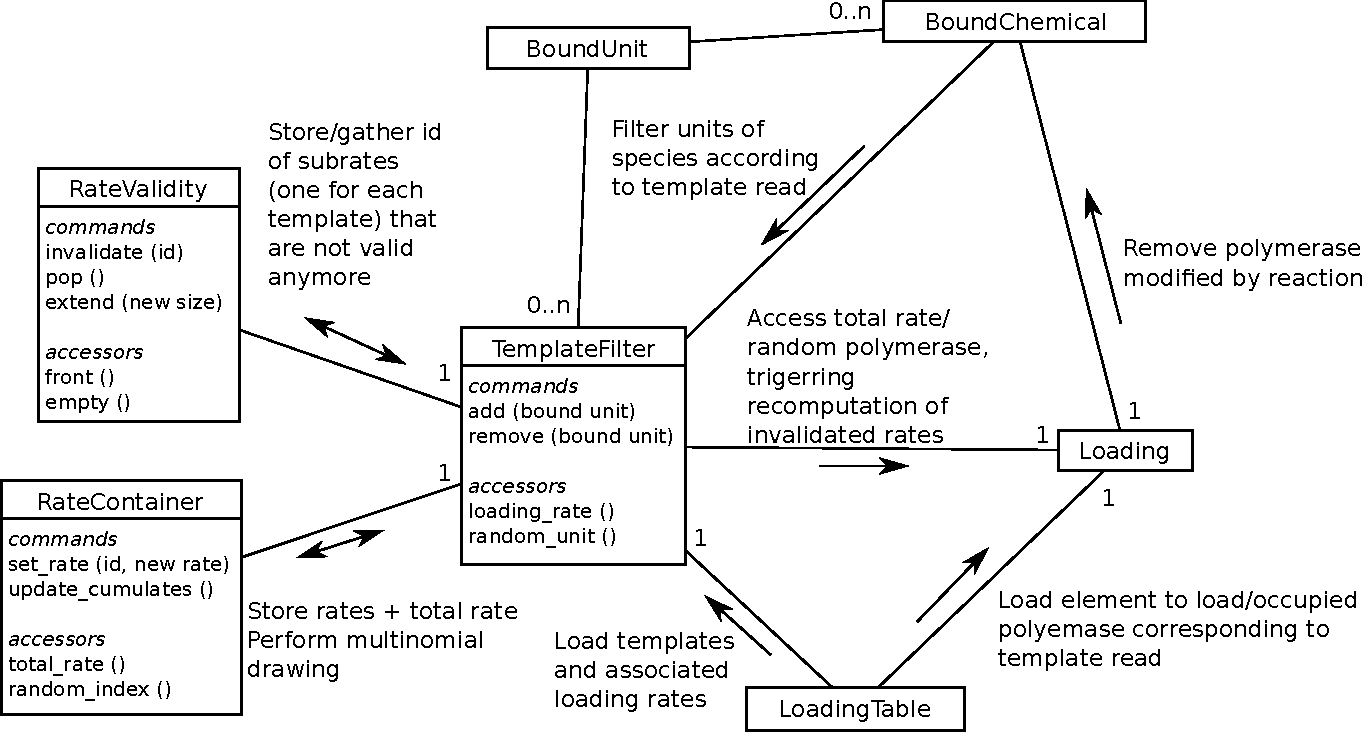
\includegraphics[width=\linewidth]{loading}
  \caption{Schematical view of the pattern used to keep subrates associated with each template up to date in a \texttt{Loading} reaction.}
  \label{fig:det_loading}
\end{figure}

\paragraph{Handling each polymerase individually} The main challenge with \texttt{Loading} is to maintain the subrates associated with each motif up to date. It needs to maintain a list of all \texttt{BoundUnit}s reading a specifing motif. To this end it uses a \texttt{TemplateFilter} (see detailed implementation of \texttt{BoundChemical}). Every time a \texttt{BoundUnit} becomes of the type of the \texttt{BoundChemical} associated with the reaction, the filter looks what motif defined in the \texttt{LoadingTable} it is currently reading. If the motif could not be found, an \texttt{UNKNOWN TEMPLATE} error message is displayed, the \texttt{BoundUnit} is not recorded in the filter and will not participate in the \texttt{Loading} reaction. The implementation is very similar to that used for \texttt{BindingSiteFamily}~\reffigp{fig:det_loading}.

\paragraph{\texttt{ProductLoading} vs \texttt{DoubleStrandLoading}} There difference between the two processes is rather small. We just added a failure condition in the case of \texttt{DoubleStrandLoading} for convenience. Depending on what reactions are used to synthesize a \texttt{DoubleStrand} it might be possible that a polymerase arrives upon a position that has already been synthesized. In this case, the \texttt{DoubleStrandLoading} fails and the polymerase is replaced by the polymerase in its stalled form.

\subsubsection{\texttt{Release}}

\paragraph{Fail polymerase (unknown product)} When a release is triggered, a \texttt{BoundUnit} from the \texttt{BoundChemical} associated with the \texttt{Release} reaction is randomly chosen. Because the \texttt{BoundUnit} knows its current position and its binding site, it will assume that product it has synthesized starts the \emph{reading frame of the binding site} and ends \emph{at the position directly preceding its current reading frame} (we assume that the polymerase translocates onto a terminating sequence which does not contribute to product synthesis). If the product is found in the \texttt{ProductTable}, everything works normally. 

If the product is not found, we display a \texttt{Unknown Product} error message but keep the simulation alive. The fail polymerase in the reaction enables the user to define a rescue pathway. If the release competes with some other reaction for the original polymerase, the fail polymerase can be the original polymerase itself. If products overlap and the polymerase was stalled due to a termination site of another product, fail polymerase can be a polymerase in a sythesizing step (\textit{e.g.} \texttt{ProductLoading}) so synthesis will resume until the next termination site is reached.


\subsection{DNA processes}
\subsubsection{DNA replication}

During exponential growth, the cell needs to duplicate its DNA content in order to proceed to division. Replication of DNA needs to be well coordinated with cell growth and division to ensure viability of the daughter cells. There are three important phases: replication initiation, elongation and termination. These phases are controlled by several (partly unknown) mechanisms to adapt to external conditions and adjust growth rate. For example, several bacteria, including \textit{E. coli} and \textit{B. subtilis}, are able to initiate replication several times during one cell cycle, so that the cell cycle can actually be shorter (down to 20 minutes) than the time needed to replicate the full chromosome (approximately 40 minutes) \citep{reyes-lamothe_chromosome_2012}.

\paragraph{Replication initiation} Replication initiation of the chromosome is an event that appears to be precisely controlled. Replication should only be initiated if growth conditions are favorable. What is more, replication should generally be triggered exactly once during cell cycle. Even in excellent growth conditions, when cells inherit a chromosome already engaged in replication, the two origins of replication fire at exactly the same time \citep{kaur_building_2014}. This implies the existence of mechanisms that inhibit replication initiation once replication has already started.

Initiation is mainly controlled by DnaA, a protein that can bind DNA in its activated form, DnaA-ATP. There are numerous DnaA binding boxes along the chromosomes, but only a few of them are essential for replication initiation. The latter are located next to the \textit{oriC} locus (Figure \ref{fig:dnaABoxes}), where the replisomes are loaded and replication actually starts. Interestingly, \textit{oriC} and the \textit{dnaA} gene are colocated in numerous bacteria \citep{briggs_chromosomal_2012}, so that the binding of DnaA inhibits its own expression, autoregulating the levels of DnaA available.

In the most simple model, DnaA polymerizes along the DnaA binding boxes, unwinding the DNA around \textit{oriC}. It is probable that this unwinding is not necessarily performed by DnaA itself. For example, in \textit{B. subtilis}, DnaA binds with DnaD, which is mainly responsible for untwisting \citep{briggs_chromosomal_2012}. Once the DNA is sufficiently untwisted, a neighboring AT-rich region, termed DNA-Unwinding Element (DUE), opens slightly, enabling loading of the first elements of the replisomes, the helicase and helicase loader (DnaC-DnaI for \textit{B. subtilis}, DnaB-DnaC for \textit{E. coli}). The position of DnaA binding boxes is not exactly conserved in different bacterial species, the loading mechanism is poorly understood. Because a loop is observed during replication initiation of \textit{B. subtilis}, \citet{briggs_chromosomal_2012} propose that DnaD is used for loop-forming and that the loop enables synchronous loading of the two replisomes (one for each direction) through DnaB (Figure \ref{fig:dnaA}, top). 

\begin{figure}[!ht]
	\centering
	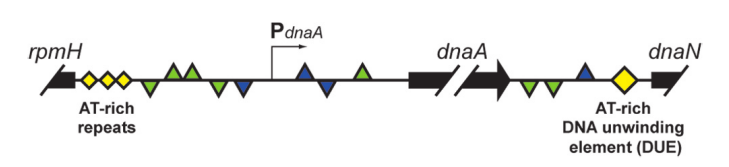
\includegraphics[width=0.49\linewidth]{figure/dnaABindingBoxes}
	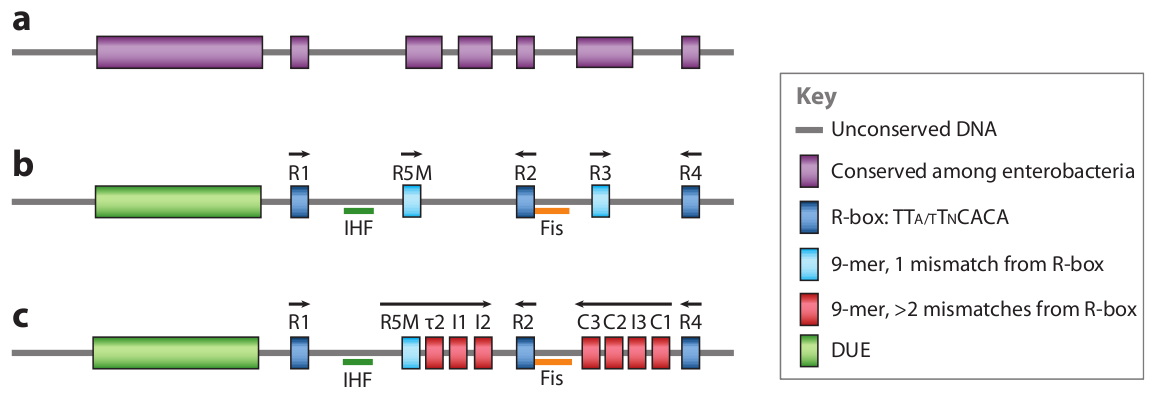
\includegraphics[width=0.49\linewidth]{figure/dnaABoxes}
	\caption{Around \textit{oriC}, several DnaA binding sites (blue and green triangles) allow for the polymerization of DnaA and, eventually, opening of the DNA at the AT-rich DNA-Unwinding Element (DUE) (left). A more detailed view shows that there are three high affinity boxes (R1, R2 and R4) that serve as nucleation points and a lot of low-affinity boxes that guide polymerization (right). Figures from \citet{leonard_regulation_2011} (right) and \citet{briggs_chromosomal_2012} (left).}
	\label{fig:dnaABoxes}
\end{figure}

Closer inspection shows that even if DnaA-ATP oligomerizes as a helix \textit{in vitro}, it may only be capable of binding ssDNA \textit{in vivo} and that the actual complex responsible for DNA unwinding also contains DnaA-ADP \citep{leonard_regulation_2011}. In this more advanced model for \textit{E. coli}, DnaA may cooperate with DNA-binding proteins IHF (integration host factor) and Fis (factor inversion stimulation) to change the 3D conformation of the origin. Several interesting points highlight that the conformation changes originate from subtle interplay between the three proteins DnaA, Fis and IHF \citep{kaur_building_2014}. (i) If none of these proteins binds DNA, the DUE opens spontaneously, while if the 3 main DnaA boxes are occupied by DnaA, it is closed. (ii) In the presence of Fis and IHF, up to two high-affinity binding boxes (R1, R2 and R4) can be deleted without impacting cell viability, while the cell dies if Fis or IHF is also removed. (iii) Fis can inhibit DnaA binding to a distance of up to 100 bp. Given these elements, it seems that the origin of replication is rather compacted, allowing all the proteins that bind in its vicinity to interact in a nucleosome-like structure (Fig. \ref{fig:dnaA}, bottom). The following ideas have been proposed \citep{leonard_regulation_2011,kaur_building_2014}: (i) Fis binds to the origin and compacts it, inhibiting DnaA binding at first, (ii) when DnaA levels are high enough, DnaA manages to bind its high affinity boxes, dislodging Fis and quickly stabilized by IHF binding and DnaA oligomerization along weak affinity boxes, (iii) the DUE opens, DnaA-ATP can bind along the ssDNA, stabilizing the opening and recruiting the helicase and helicase-loader.

\begin{figure}[!ht]
	\centering
	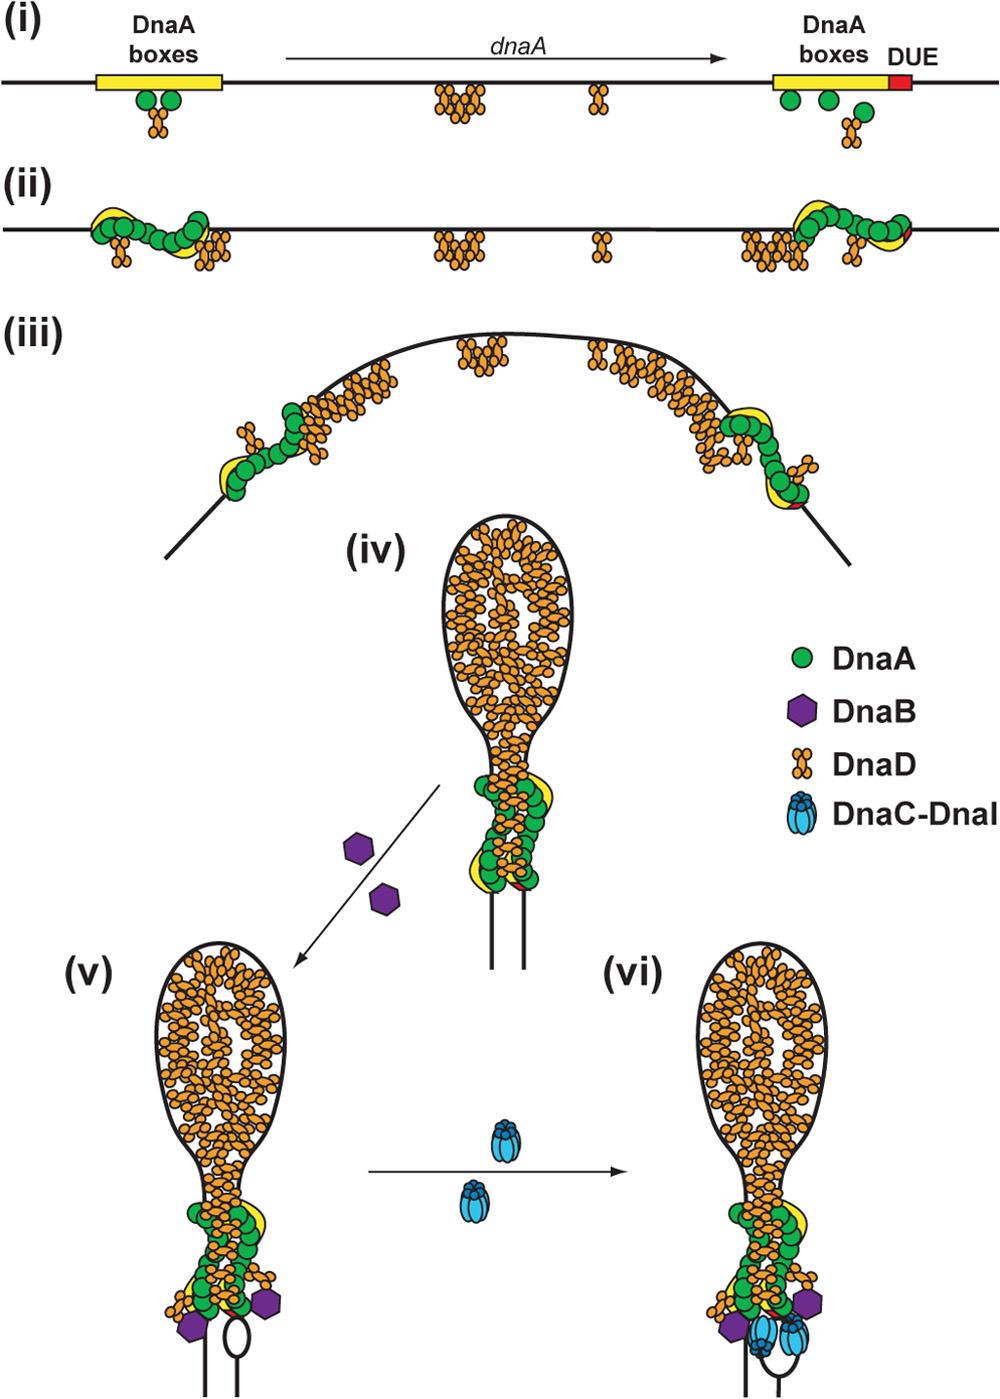
\includegraphics[width=0.5\linewidth]{figure/dnaAPolymerizationModel}
	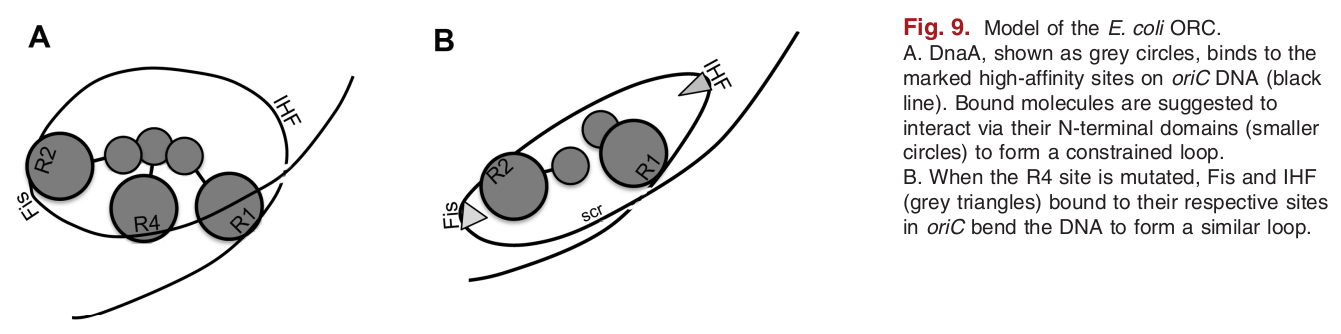
\includegraphics[width=0.8\linewidth]{figure/dnaA3DModel}
	\caption{Control of DNA replication through DnaA proteins and other helper proteins in \textit{E. coli} and \textit{B. subtilis}. Top: Model for replisome loading by helper proteins in \textit{B. subtilis}. DnaD accelerates DnaA binding and its unwinding and polymerization activities form a loop. Finally DnaB is recruited on each end on the loop, each DnaB loading a helicase DnaC on one of the strands with the help of helicase-loader DnaI. Bottom: Similar model for \textit{E. coli}, where loop forming occurs cooperatively between DnaA and DNA binding proteins Fis and IHF. Figures from \citet{briggs_chromosomal_2012} (top) and \citep{kaur_building_2014} (bottom).}
	\label{fig:dnaA}
\end{figure}

How initiation is controlled is largely unknown and may be species specific. For example, \textit{E. coli} does not have homologs for \textit{B. subtilis} DnaB and DnaD proteins (\textit{E. coli} DnaB and DnaC are the homologs of \textit{B. subtilis} DnaC and DnaI, respectively). As a result, the initiation is strongly dependent on DnaA-ATP levels in \textit{E. coli} but less in \textit{B. subtilis}, where DnaB and DnaD seem more critical \citep{briggs_chromosomal_2012}. In \textit{E. coli}, it is estimated that around 20 DnaA-ATP are needed for intiation, the cell containing 1000 to 2000 DnaA molecules \citep{leonard_regulation_2011}. DnaA-ATP levels are controlled by several mechanisms \citep{leonard_regulation_2011}:
\begin{itemize}
	\item Newly synthesized DnaA has a higher affinity for ATP. If levels of ATP are high compared to ADP, there is high probability that it will associate with ATP.
	\item Regulatory Inactivation of DnaA (RIDA): the replisome contains processivity $\beta$-clamps (see below), that bind to proteins that hydrolize DnaA-ATP (in \textit{B. subtilis}, a similar role is played by YabA, except it does not hydrolyze DnaA-ATP, it favors colocalization of DnaA-ATP with the replisome).
	\item Once replication has started, the number of DnaA binding sites rapidly increases, diluting remaining DnaA-ATP, notably the \textit{datA} locus, which contains 3 high affinity DnaA binding sites. 60 to 300 proteins can bind to this locus which is replicated at approximately 1/3rd of the cell cycle.
	\item DnaA Recharging Sites (DARS): loci which bind 3 DnaA-ADP and converts them to DnaA-ATP by an unknown mechanism (only 2 DARS loci have been uncovered). Membrane based processes could also be involved in DnaA recharging.
\end{itemize}
What is more, a sequestration protein SeqA may bind the low-affinity DnaA binding boxes during one third of the cell cycle after initiation, avoiding DnaA rebinding. In mutant cells lacking SeqA, replication reinitiates immediatly \citep{leonard_regulation_2011} A similar mechanism for \textit{B. subtilis} could be the ParAB-\textit{parS} system \citep{reyes-lamothe_chromosome_2012}. This system, probably responsible for chromsome segregation (see below), binds to the \textit{parS} locus through parB. It seems that ParA binds DnaA and influences replication initiation, maybe because ParB hydrolyzes ParA, complexing ParB-\textit{parS} to the \textit{oriC}, this association being stabilized by SMC proteins. The complex can then migrate towards one of the cell poles and it is possible that it may be unavailable for reinitiation during that time. Taking into account all these elements, \citet{leonard_regulation_2011} propose a model for DnaA titration that could partly regulate replication initiation (Fig. \ref{fig:dnaATitration}).

\begin{figure}[!ht]
	\centering
	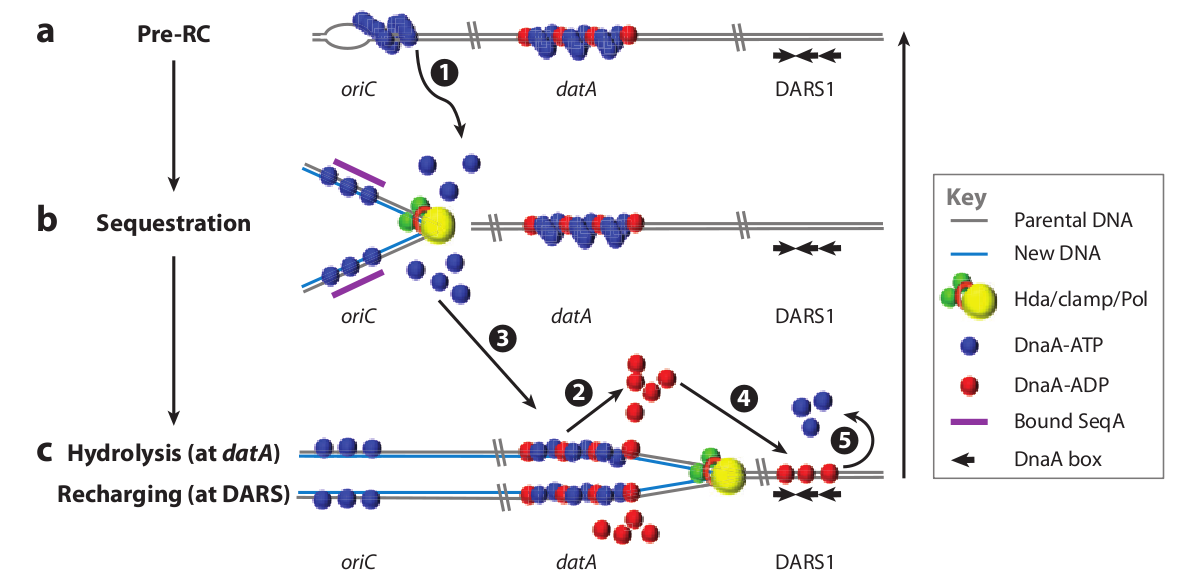
\includegraphics[width=0.8\linewidth]{figure/dnaASequestrationModel}
	\caption{Titration of DnaA levels. Once Dna-ATP levels are high enough next to the \textit{oriC}, replication initiates and displaces most of the DnaA molecules (a). SeqA binds on the low affinity binding sites next to \textit{oriC}, so displaced DnaA-ATP cannot rebind and maybe clusters around \textit{datA} (b). Hda protein, associated with the $\beta$-clamp of the replisome, may hydrolyze DnaA-ATP when the replisome goes through \textit{datA}. Dna-ATP is regenerated thanks to DARS loci and slowly becomes available again for replication initiation (c). Figure from \citet{leonard_regulation_2011}.}
	\label{fig:dnaATitration}
\end{figure}

Even though our understanding of the initiation of replication on the chromosome is somewhat limited, experiments show that it is strictly controlled by the cell. On the other hand, the replication of other DNA elements such as plasmids is not as severely controlled, as their exact number within the cell can vary. Initiation is not triggered by DnaA but by other proteins or RNAs that are plasmid-specific. Shortly, there are two main types of plasmids in a bacterial cell: large plasmids present in low copy numbers and small plasmids present in high copy numbers (Figure \ref{fig:plasmidInitiation}). The large plasmids have a similar initiation system as the chromosome, triggered by a DNA binding protein coded by the plasmid itself (generically called Rep). Initiation is probably regulated by the copy number of plasmids, either through a RNA coded by the plasmid that blocks the synthesis of Rep, or simply because Rep is able to polymerize at high concentrations, becoming unavailable for initiation. In small plasmids, initiation is probably controlled by a RNA and DNA polymerase I. The RNA (termed RNAII) slightly opens the double helix and binds to DNA, acting as a primer for DNA polymerase I, which further opens DNA. A single replisome can then be loaded on the other strand (in this case, replication is unidirectional). Copy number is probably controlled by another RNA (termed RNAI), which interfers with RNAII at sufficiently high concentrations.

\begin{figure}[!ht]
	\centering
	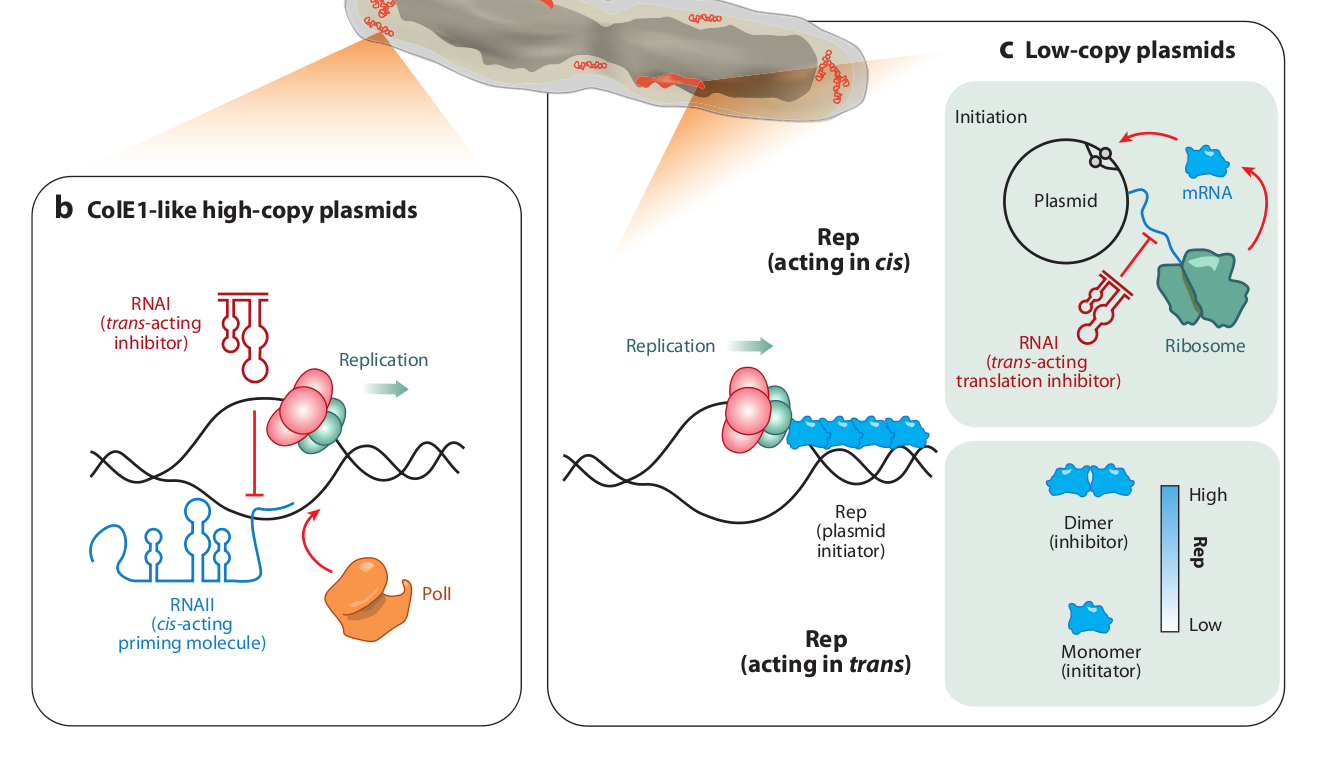
\includegraphics[width=0.8\linewidth]{figure/plasmidReplicationInitiation}
	\caption{Plasmid replication follows similar principles as chromosome replication (it uses the same replisome). However, initiation is regulated by plasmid specific elements. Small plasmids probably use RNAs to initiate (RNAII) and inhibit (RNAI) replication. Large plasmids use a protein that acts similarly to DnaA and which is regulated by the plasmid copy number. Figure from \citet{reyes-lamothe_chromosome_2012}}.
	\label{fig:plasmidInitiation}
\end{figure}

\paragraph{Replication elongation} Once replication is initiated, helicases are loaded upon the DNA strands, one in each direction (see above). From the helicases, the whole replisome complex can be loaded and start polymerizing DNA. The replisome ensures processivity and rapid replication of the whole chromosome, as well as synchronous replication of the leading strand and the lagging strand. Indeed, DNA polymerases are only able to assemble DNA in the 5' to 3' sense, which corresponds to the direction the leading strand is processed, but antisense to lagging strand processing. Therefore, the leading strand is easily handled while replication of the lagging strand is handled by loop forming that allows for fragment-wise replication of a few kbs of DNA (termed Okazaki fragment).

The composition of the replication reflects these different tasks (Figure \ref{fig:replisome}). The helicase DnaB (DnaC for \textit{B. subtilis}) is formed of a hexamer that separates the DNA, forming the replication fork. Bound to the helicases, three primases DnaG stabilize the helicase structure and cooperate for synthesis of short RNA sequences on the lagging strand called primers used to initiate Okazaki fragments. Finally, a clamp loader bound to the helicase is responsible for recruiting DNA polymerases and $\beta$-clamps. The number of DNA polymerases can vary depending on the number of subunits $\tau$ in the clamp loader \citep{reyes-lamothe_chromosome_2012,stratmann_dna_2014}: replisomes with 2 or 3 associated DNA polymerases have been observed, the latter seemingly more efficient. The nature of DNA polymerases is also unclear: it seems that in \textit{E. coli} Pol III is preferentially recruited because of its high fidelity, while in \textit{B. subtilis} two different polymerases may be used for the leading and the lagging strand \citep{reyes-lamothe_chromosome_2012,stratmann_dna_2014}. The recruitment of $\beta$-clamps is also essential as it binds to DNA polymerases and increases their processivity from a few nucleotides to several tenths of kb \citep{reyes-lamothe_chromosome_2012}. Because these elements are bound to the clamp loader, they are efficiently recycled, allowing for very fast replication.
\begin{figure}[!ht]
	\centering
	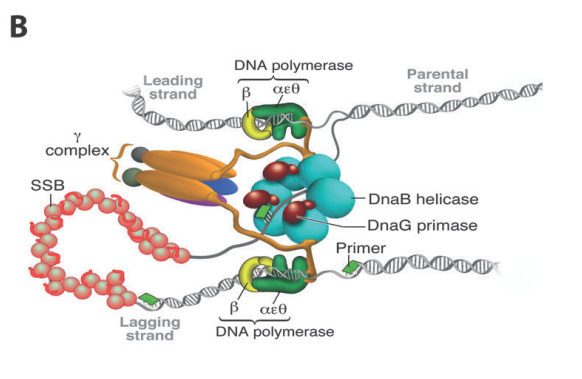
\includegraphics[width=0.6\linewidth]{figure/replisome}
	\caption{Standard bacterial replisome stucture (as reconstructed from \textit{E. coli}). Figure from \citet{stratmann_dna_2014}.}
	\label{fig:replisome}
\end{figure}

Coordination of leading and lagging strand replication is not fully understood. As replication occurs continuously on the leading strand, it seems intuitive that replication should occur more rapidly than on the lagging strand or that the loop forming/relase of Okazaki fragments has to be particularly efficient. Two models have been proposed for the loop forming process: the collision process and the signaling process (Figure \ref{fig:replisomeElongation}, left). In both models, DNA polymerase starts from a primer, progressively forming a loop as ssDNA (protected by SSB) and recently polymerized DNA accumulate between the fork and the DNA polymerase. In the collision model, the DNA polymerase proceeds until the next Okazaki fragment, stalling and becoming available for elongation from the next primer. If a primer is ready before the current fragment is finished, the fork could pause, making this process quite inefficient. In the signalling model, the DNA polymerase is reused as soon as a primer is ready, so that a lot of fragments remain incomplete, containing large portions of ssDNA. In fact, the presence of 3 polymerases indicates that the reality might be in-between, explaining how the lagging strand synthesis can be as efficient as the leading strand synthesis (Figure \ref{fig:replisomeElongation}) \citep{stratmann_dna_2014,duderstadt_replication-fork_2014}. With 3 polymerases, 2 polymerases might be synthesizing at the same time, one finishing the previous fragment while the other one is available for recruitment on a new primer. As a matter of fact, it is also highly probable that the replisome is very dynamic, with frequent recruitment and detachment of primases and polymerases. In this way, even a 2 polymerase replisome could operate in a similar manner, by periodically detaching polymerases to finish a fragment and recruiting a new polymerase at the replisome. This remains to investigate but seems pretty likely as numerous polymerases gravitate around the replisome and such exchanges have been observed on the leading strand \citep{stratmann_dna_2014}.
\begin{figure}[!ht]
	\centering
	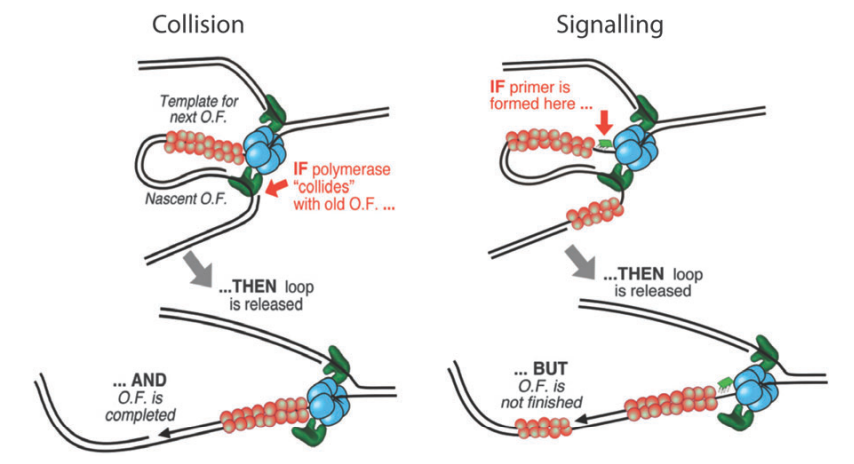
\includegraphics[width=0.49\linewidth]{figure/replisomeElongation}
	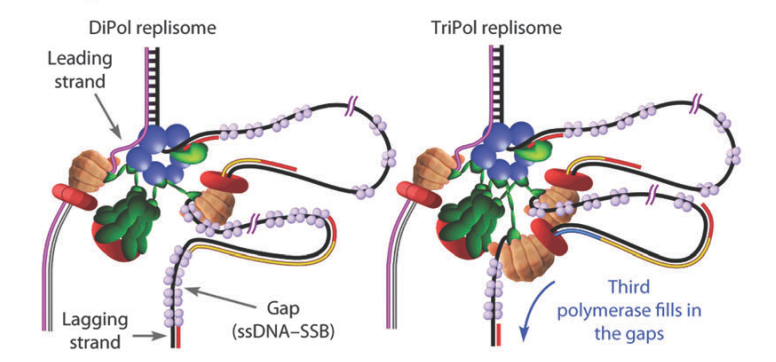
\includegraphics[width=0.49\linewidth]{figure/replisomeThreePolymerases}
	\caption{Elongation models for the lagging strand (left). Likely elongation according to recent experiments that mixes the two previous models (right). Figure from \citet{stratmann_dna_2014}.}
	\label{fig:replisomeElongation}
\end{figure}

Some details of elongation remain unclear. RNA primers have to be removed, resynthesized and ligated by specific polymerases, but the coordination with the replisome has not been investigated (to our knowledge). The cooperation with SMC molecules or obstacle management is known to exist but very little is known. Some elements are presented in the repair section, where stalling of the replisome is handled by RecA and restarting of replication is handled by a specific primosome complex. However, it is unknown if the replisome collapses, helps recruiting repair proteins or lower fidelity polymerases that can bypass some specific DNA damages.

\paragraph{Replication termination} Termination of replication occurs in the \textit{terC} region thanks to Tus proteins. These proteins are able to block a replisome along one direction. Replisomes will thus meet along a small segment delimited by two Tus proteins in opposite directions, probably even at the site of one of these proteins. The length of the two replicons is thus not totally fixed but limited to a certain range.


\paragraph{Computational representation}
See illustration how the cell chromosome is used. Some more information may be needed TBD.
When a chromosome is fully duplicated (when the first column of the cell chromosome only contains -2), the process consists of deleting the current chromosome and creating 2 new ones with the correct initialization. TBD do we clean the chromosomes? Typically, when the chromosome was manipulated.

Needs also other things but from the DNA point of view, there seems to have enough information.

\subsubsection{DNA movement}
\textcolor[rgb]{1.00,0.00,0.00}{What do we do when a gene change of volume due to condensation or segregation for example. Normally, a matter of changing the number of the volume in the cell chromosome and the corresponding volume chromosomes. But assume that anything that is currently binded to the DNA is the property of the DNA and was 'erased' from everywhere else. Also assume that volume chromosome only contains the strictly necessary information about the DNA in the volume and that it is a state with changing size.}

\subsubsection{DNA manipulations}
\paragraph{Codon aggregation damage}
\textcolor[rgb]{1.00,0.00,0.00}{Gap site, Abasic site, Sugar-phosphate, Base, Intrastrand cross link, Strand break, Holliday junction}
DNA is subject to numerous forms of damage that can be either endogenous or exogenous. They can result in chemical modifications of some bases, in single strand breakage (missing of one base on one of the strands), double strand breakage or cross links between DNA strands. Chemical modifications can originate from different type of radiations (UV, x-rays, etc.), drugs or reactants naturally present in the cell leading to alkylations, oxydations, deaminations, etc. Another important source of DNA mismatches is the replication machinery itself which can make use of the wrong dNTP (dUTP for example).

DNA modification is one of the prerequisites to evolution. DNA mutations lead to the development of novel functions, regulatory systems, etc. However, replication fidelity is also essential for selection and conservation of important existent functions. There is a trade-off between these two aspects that is well illustrated in \textit{B. subtilis} by the existence of efficient repair mechanism on the one hand and some DNA polymerases that favor propagation of some types of damage (such as DnaE) on the other hand.



\paragraph{Codon aggregation insertion}
Insertion of one (or several) lines in the DNA states.

\paragraph{Codon aggregation deletion}
Putting 0 in the corresponding places and not deletion of the line(s) because a codon aggregation can be deleted in a fork.

\paragraph{Codon aggregation repair}
There are several pathways employed for DNA repair corresponding to the type of damage undergone.

\subparagraph{Mismatch Repair (MMR)} This pathway is dedicated to reparation of base mismatches. In \textit{E. coli}, repairing is initiated by MutS (Sensor) which detects the mismatch and MutL (Linker) which recruits further proteins. The endonuclease MutH then nicks the DNA next to the mismatch enabling the helicase and exonuclase UvrD to remove bases around the mismatch. The resulting gap is filled in by DNA polymerase III and DNA Ligase. The newly synthesized strand is specifically targeted by these proteins thanks to the methylase Dam used for marking the original strand. In \textit{B. subtilis}, only MutS and MutL seem to be conserved (MutL having an additional endonuclease activity). Recognition of the newly synthesized strand could be linked to a strong coupling of MMR with replication and colocalization with the replisome.

\subparagraph{Base excision repair (BER)} The BER pathway repairs most non-bulky base modifications such as oxydations, deaminations, UTP incorporation, etc. Schematically, glycosylases detect the lesion, remove the damaged base, endonucleases then nick the DNA next to the missing base so that exonucleases remove some bases on the strand around the missing base. The small gap is then closed by a repair DNA polymerase (such as Polymerase I) and ligated by a DNA ligase. For example, in \textit{B. subtilis}, the glycosylases MutM and MutY (part of the GO system) detect oxidized Guanine to avoid its pairing up with dATP. Another example is Uracil DNA-glycosylase, which removes dUMP from DNA. 

\subparagraph{Nucleotide excision repair (NER)} The NER pathway is very similar to the BER pathway, except that it repairs bulky lesions caused by UV radiations or drugs. This pathway is highly conserved and partly regulated by the SOS response (mediated by RecA). The UvrABC complex is responsible for detecting the damaged base and nicking the DNA at surrounding bases. Helicase UvrD removes the nicked segment. Finally, DNA Pol. I and DNA ligase restore the missing segment.

\subparagraph{Alkylation damage} There are specific pathways that address alkylation (such as methylations). \textit{B. subtilis}, as a soil-living bacterium, is particularly exposed to alkylating agents. There are at least three pathways responsible for repairing alkylated bases: two pathways based on glycosylases (one being constitutive, the other inducible) and one pathway based on alkyltransferases (enzymes that suicide by transferring the alkyl group onto themselves).

\subparagraph{Homologous recombination (HR)} During replication, double strand breaks (DSB) can be repaired by using the other copy of the chromosome (Figure \ref{fig:HR}). First, the DSB is stabilized by RecN and digested by protein complexes (AddAB and RecQSJ in \textit{B. subtilis}) that create hangovers of single stranded DNA (ssDNA) on the 3' strands. RecA binds to the ssDNA (probably with the help of the RecFOR complex that prevents SSB from binding). RecA, activated by ATP or dATP, enables invasion of the sister chromosome at a homologous sequence, creating a D-loop where one of the broken 3' strands is inserted and forming Holliday Junctions between the two chromosomes. DNA elongation occurs from the 3' strand and the Holliday Junctions are cleaved by RecU (or a homologous protein).

There is a variation if the DSB caused the replication to stall (Figure \ref{fig:HR}, right). This situation may occur if a single-strand break is present on the original chromosome which becomes a DSB after passage of the replication fork. In this case, there is only one DNA end to digest and the invasion leads to only one Holliday Junction. The primosome complex, composed of Pri and Dna proteins, detects the D-loop and helps loading the replisome to resume replication. It seems that several Structural Maintenance of Chromosome (SMC) proteins are involved throughout the process (such as RecN), but their role is not clearly elucidated.

\begin{figure}[!ht]
\centering
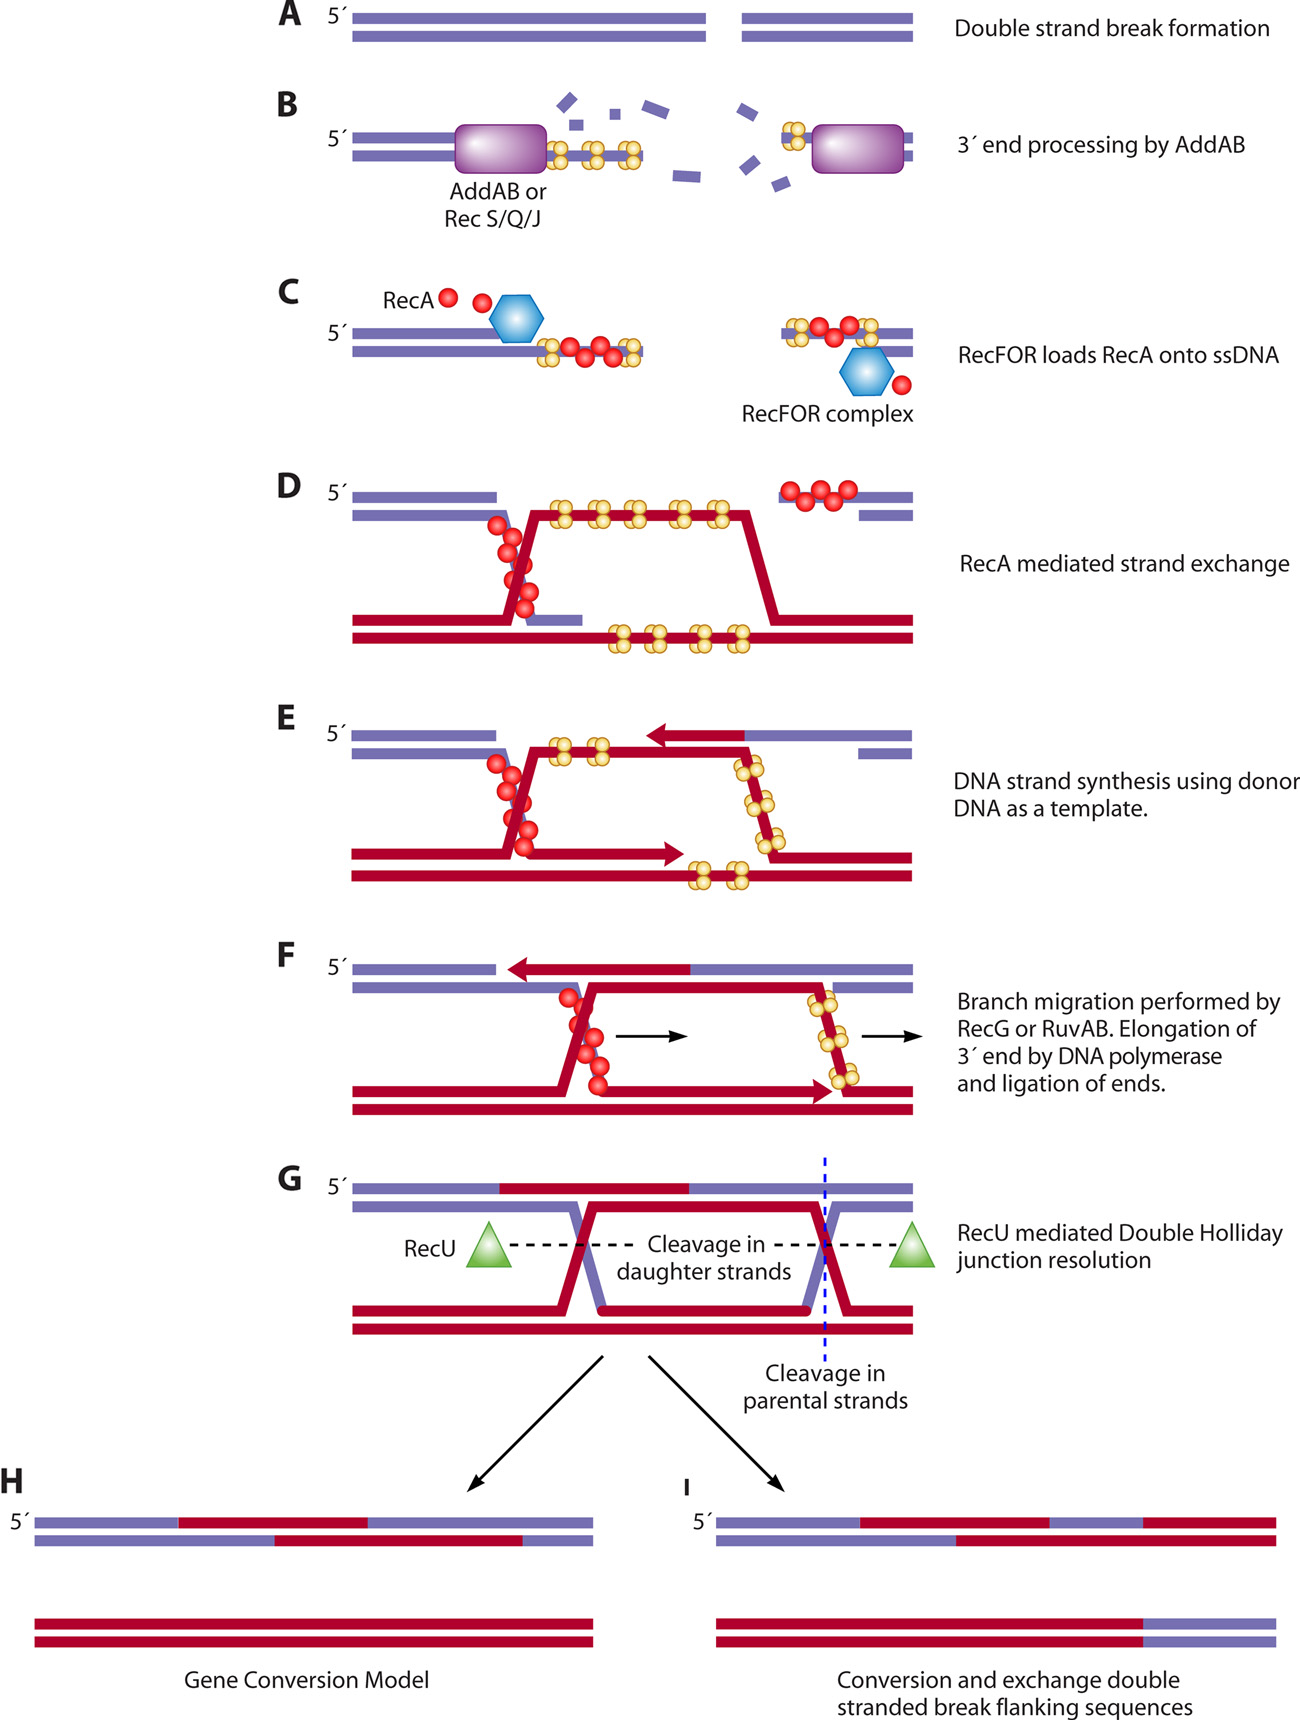
\includegraphics[width=0.54\linewidth]{figure/HR1}
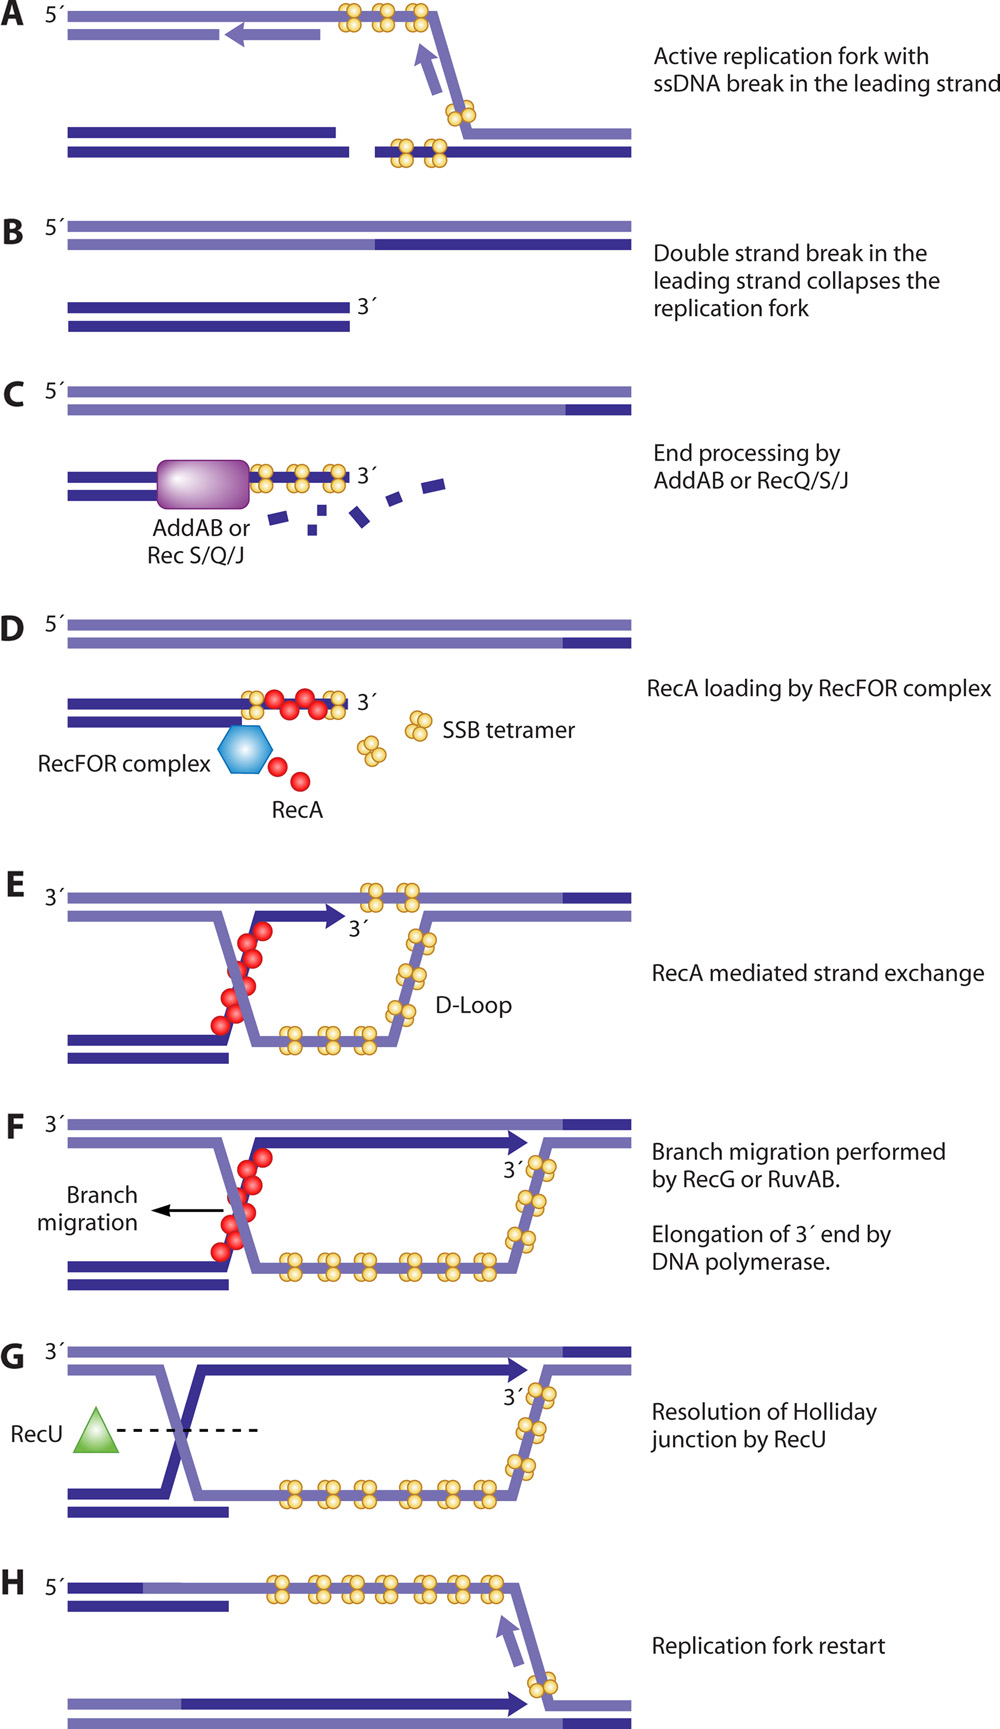
\includegraphics[width=0.44\linewidth]{figure/HR2}
\caption{Homologous recombination and repair of DSB in \textit{B. subtilis} in the general case (left) and when the DSB appears in the replication fork (right). From Lenhart \textit{et al.}.}
\label{fig:HR}
\end{figure}

\subparagraph{Nonhomologous end joining (NHEJ)} This pathway is also responsible for DSB repairing but it is less efficient than homologous recombination. It is used when there is no other copy of the chromosome present in the cell. As in HR, a protein (probably YkoV for \textit{B. subtilis}) binds the DSB and favors recruitment of another protein (LigD like, probably YkoU for \textit{B. subtilis}) that is able to perform exonucleation, polymerisation and ligation. The mechanisms are not totally clear but it seems that because LigD is able to perform these 3 functions, no other protein is needed. However, some bases need to be deleted and repolymerized during the reparation, possibly leading to DNA losses or insertions, making NHEJ a low-fidelity repair mechanism.


\subsubsection{DNA compaction}
DNA compaction occurs through various proteins that are able to clamp the DNA together, forming high-densitiy bundles, leading to a compact form within the cell called a nucleoid. The compaction is due to supercoiling generated by DNA gyrase and topoisomerases, the action of histone-like proteins (HU, IHF, Fis H-NS) and SMC proteins (SMC-ScpA-ScpB for \textit{B. subtilis}, MukBEF for \textit{E. coli})(Fig. \ref{fig:compaction}). According to several studies, the nucleoid adopts a large helical structure composed of two intertwined branches, at least during G1 phase (Fig. \ref{fig:compaction}) \citep{berlatzky_spatial_2008, ptacin_chromosome_2013, fisher_four-dimensional_2013}. This structure is dynamical, with specific loci moving of about 10\% of cell length within a few seconds \citep{wiggins_strong_2010,fisher_four-dimensional_2013} and seems to be ATP-dependent \citep{fisher_four-dimensional_2013,weber_nonthermal_2012}. \citet{fisher_four-dimensional_2013} identify these variations as waves that could be used to unbind some of the DNA binding proteins, avoiding overcondensation, unwanted linkage between loci and facilitating segregation. In general, it seems that the chromosome is linearly organized around the \textit{oriC}, meaning that the bundling occurs progressively, so that the position within the cell reflects the position along the chromosome \citep{wiggins_strong_2010}.
\textcolor[rgb]{1.00,0.00,0.00}{Condensation, ”clamping” of the DNA by structural maintenance of chromosome (SMC) proteins, supercoiling, macromolecular crowding, charge neuralization?}
If spatialization is used, condensation and segragation might be modelled directly. Supercoiling needs another state.
\textcolor[rgb]{1.00,0.00,0.00}{Compactation should also impact the accessibility of the chromosome.}

\begin{figure}[!ht]
	\centering
	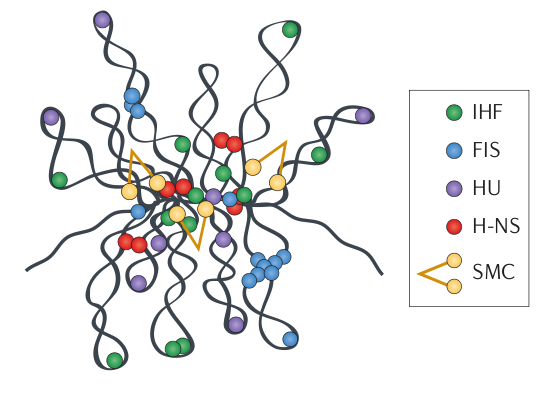
\includegraphics[width=0.4\linewidth]{figure/SMC.png}
	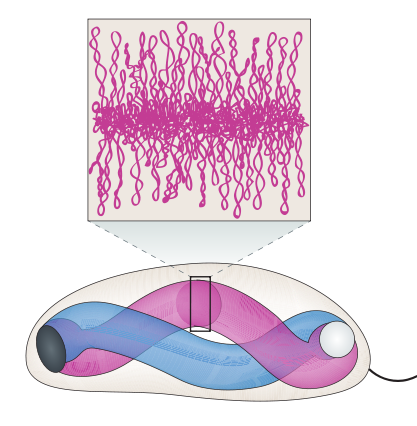
\includegraphics[width=0.4\linewidth]{figure/compaction.png}
	\caption{Proteins responsible for chromosome compaction (left) and model for nucleoid organization in \textit{C. crescentus} (right). Figures from \citet{wang_organization_2013}.}
	\label{fig:compaction}
\end{figure}

\subsubsection{DNA segregation}
As replication proceeds, sister chromosomes/plasmids have to be separated in order to allow proper cell division. This process is also largely unknown, but several models based on experiments have been proposed, it seems that there is no universal solution valid for all bacteria. There are two main challenges: unlinking the chromosomes and driving them to opposite poles of the cell.

Unlinking is generally done at the replisome level. Supercoiling accumulates at the front of the helicase due to its unwinding activity. This supercoiling can be physically propagated to the back of the replisome, creating an entanglement between sister chromosomes. The DNA gyrase limits this propagation by diminishing supercoiling at the front of the replisome, while Topoisomerase IV disentangles the chromosome copies \citep{reyes-lamothe_chromosome_2012}.

Segregation can be done according to several mechanisms, particularly for plasmids. For high copy number plasmids, it is possible that segregation occurs purely through diffusion. For other plasmids, elements of the cytoskeleton can be used to separate the copies (Figure \ref{fig:dnaMigration}ab). ParR proteins may bind to \textit{parC} loci on the plasmid and serve as a basis for actin-like ParM that polymerizes between the copies, progressively seperating them. Similarly, TubR might bind to \textit{tubC} and migrate along filaments of tubulin-like TubZ. The last mechanism may target plasmids as well as the chromosomes (Figure \ref{fig:dnaMigration}c). It is also composed of a DNA binding protein ParB, binding to \textit{parS} (close to \textit{oriC}), and a motor protein ParA. However, ParA attracts ParB only in its activated and DNA-binding form ParA-ATP, probably located along the nucleoid. ParB hydrolises ParA-ATP, releasing it in the cytosol until it gets reactivated and rebinds DNA away from ParB. In this way the two ParB-\textit{parS}-\textit{oriC} complexes migrate in opposite directions until steady-state is reached, with equivalent ParA-ATP pools located on each side of each complex (approximately at the quarter of each pole). It seems that this system works cooperatively with SMC proteins, but the details are yet unknown \citep{reyes-lamothe_chromosome_2012}. Another possibility is radial stress \citep{fisher_four-dimensional_2013}. Sister chromatides are bundled separately but hold together by some tether. They accumulate at the center of the cell, along with the mother DNA, which is bundled separately. The mother DNA pushes the two growing chromatides aside with a force that gets stronger for sterical reasons until the tethers break and the chromatides migrate towards the poles. According to \citet{fisher_four-dimensional_2013}, this phenomenon happens up to four times during segregation. The main idea here is that segregation results from efficient bundling of neosynthesized DNA, so that mother DNA and sister chromatides form 3 very distinct structures that repel each other but are linked by tethers.
\begin{figure}[!ht]
	\centering
	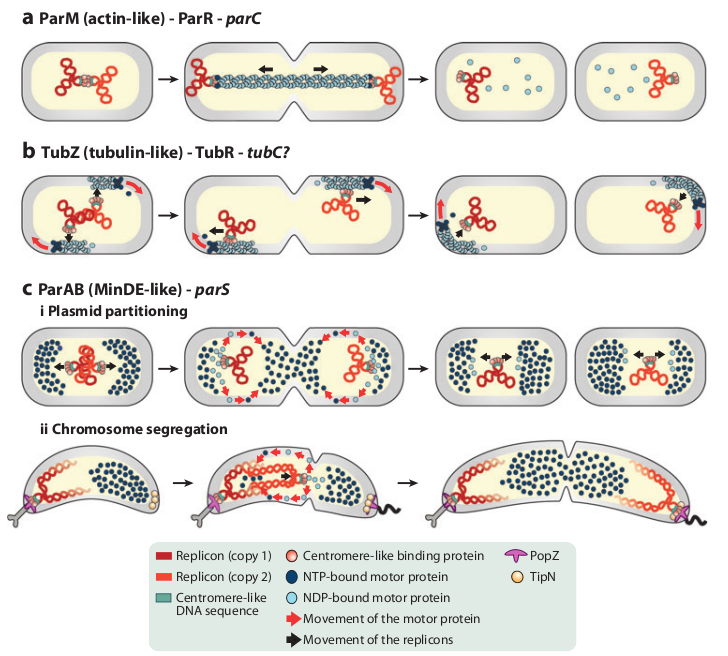
\includegraphics[width=0.8\linewidth]{figure/DNAmigration}
	\caption{Migration of plasmids and chromosome can be mediated by different systems. It can be based on elements of the cytoskeleton: separation through polymerization of actin-like proteins (a), migration along tubulin-like proteins (b). Alternatively, migration may based on an oscillatory system, where activated proteins (ParA-ATP) attracts another protein (ParB) linked to the plasmid or chromosome (\textit{parS} loci) that hydrolises it (c). DNA migration is then controlled by the location of pools of activated proteins. Figure from \citet{reyes-lamothe_chromosome_2012}.}
	\label{fig:dnaMigration}
\end{figure}

Similar to initial segregation, final segregation includes decatanation of two chromosomes and migration of the \textit{ter} region to the two poles, but it is assisted by a new protein and associated with the formation of the FtsZ ring at the septum. The FtsZ ring cannot polymerize as long as the nucleoid is located at the center of the cell. Cytokinesis thus begins when the initial migration of DNA copies is already advanced. Once FtsZ ring forms, the DNA translocase FtsK (SftA in \textit{B. subtilis}) is recruited by the divisome to the membrane next to the FtsZ ring. FtsK seems to coordinate several actions in the final segregation. FtsK binds to \textit{dif} loci next to the \textit{ter} regions, aligning the \textit{ter} region with the septum. FtsK can also translocate remaining DNA at the final stages of septum closing. FtsK also cooperates with Xer proteins to separate chromosomes copies that might have merged due to recombination by creating a Holliday junction.
 

\subsubsection{DNA transformation}

DNA transformation is the incorporation of extracellular DNA into the cell. The role of transformation is not totally understood. Most probably, it allows for generation of bacterial sex and generation of an enhanced genetic diversity in changing environments or stress situation. The master regulator of competence ComK induces more than 150 genes, 30 of which only are known to be directly involved in DNA transformation.

Transformation uses the recombination machinery to integrate the DNA into its own genetic material. Numerous proteins of the SOS response are therefore involved but it seems that the induction of these proteins is mediated by ComK, the master regulator of competence state, and is LexA-independent~\citep{kidane_cell_2012}. DNA transformation is only activated in specific physiological conditions by quorum sensing. ComX and the Competence and Sporulation Factor are secreted, activating ComP-ComA transduction. More than 150 genes are then directly or indirectly induced, including the DNA translocation machinery and the recombination machinery~\citep{kidane_cell_2012}.

The DNA translocation machinery assembles towards the cell pole and is composed of three groups \citep{kidane_cell_2012}:
\begin{itemize}
	\item The first group is responsible for binding dsDNA and transforming it into ssDNA. Known proteins are from the ComG family (ComGA, ComGC, ComGD, ComGE, ComGG) that form a pseudopilus able to drag DNA toward the membrane and NucA, which fragments dsDNA, allowing it to be digested to ssDNA by an unknown enzyme.
	\item The second group translocates ssDNA into the cell. It is composed of proteins from the ComE and ComF families (ComFA, ComEA, ComEC, maybe ComFB, ComFC, ComEB). The junction with the first group is done by ComFA and ComGA.
	\item The last group binds DNA inside the cell and performs its integration. It is composed of the induced proteins DprA, SsbA, SsbB, CoiA, RecA and the constiutive proteins RecU and RecX. Its association with the rest of the translocation machinery is highly dynamic.
\end{itemize}
Once the ssDNA is translocated within the cell, the third group protects it from degradation and recruits protein that are also involved in classical homologous recombination:
\begin{itemize}
	\item SsbA and SsbB bind and protect ssDNA from degradation.
	\item RecN and SsbE stabilize the ends of the DNA.
	\item DprA and RecO destabilize the SSB proteins and allow RecA loading.
	\item RecA loading is regulated by RecF, RecX and RecU.
\end{itemize}
Once RecA is loaded along the ssDNA, it forms a compact filament that is driven towards the center of the cell. It may be integrated within the genome if it is homologous to an endogeneous sequence (with a probability of up to 40\%~\citep{kidane_cell_2012}) or may be transformed into a plasmid if it has a primosome assembly site (\textit{pas})~\citep{kidane_cell_2012}. If a homologous sequence is found, an invasion similar to Homologous Recombination occurs (see DNA repair process). However, branch migration is not fully understood and HJ resolution may not be mediated by RecU, contrary to classical homologous recombination.

Formation of new plasmid is a little more complex as it may occur according to different mechanisms that are species specific. \citet{kidane_cell_2012} list three possibilites that could contribute to plasmid creation for ssDNA containing a \textit{pas} sequence:
\begin{itemize}
	\item Plasmid facilitation: the ssDNA transiently binds to the chromosome, forming a loop that is replicated using the free ends of the ssDNA as primers, closing the loop by adding chromosomal DNA to the ssDNA.
	\item Plasmid transformation (necessitates internal homologies): in the absence of homology, RecA unbinds and the ssDNA is converted to dsDNA thanks to his \textit{pas}. It is then circularized based on its internal homologies.
	\item Monomeric activation: poorly understood process that could work even without internal homologies. Does not seem to exist in \textit{B. subtilis}.
\end{itemize}


\subsection{Transcription}
Not detailed but would works like translation. 

\textcolor[rgb]{1.00,0.00,0.00}{Non coding DNA?}

\subsection{Translation}
See mRNA state for evolution.

\subsection{RNA processes}

\subsubsection{RNA processing}

Some polycistronic RNAs have to be cleaved before they become functional. This may be the case for some mRNAs, but is typical for sRNAs, tRNAs and rRNAs. The 30S RNA transcript of \textit{E. coli} undergoes several rounds of cleaving performed by different ribonucleases yielding a 9S, pre 16/17S and pre-23S intermediate before obtaining the 5S, 16S and 23S rRNA \citep{arraiano_critical_2010}. tRNAs also have to be cleaved at 3' 5' ends by a similar process involving several ribonucleases \citep{arraiano_critical_2010}. As for sRNA, their processing is globally unknown, except for a few examples.
\textcolor{red}{What level of detail do we want ?}

\subsubsection{RNA modifications}

\textcolor{red}{According to Karr, some bases of the RNAs are modified for proper folding and better coding recognition, but we have little data about it.}

\subsubsection{RNA decay}

There are two sides to RNA decay: the degradation machinery and possible determinants for targetting specific mRNA degradation. Let us start with the degradation machinery. There are numerous proteins that are able to cleave RNAs, some are more involved in RNA processing, some in degradation, but there is a large overlap in these activities \citep{arraiano_critical_2010}. We are only going to focus on the main ribonucleases generally considered as being responsible for global RNA degradation.

In \textit{E. coli}, the main enzyme is RNase E, an endonuclease that initiates degradation of RNAs. It seems to have two recognition pathways. Either the RNA has been modified on its 5'-end by the pyrophosphohydrolase RppH from 5' PPP to 5'P, enabling docking of the RNA by RNase E, or it may be recognized by associating with the C-terminal domain of RNase E, possibly using intermediates \citep{laalami_initiation_2013}. The latter case is not totally understood, numerous cofactors such as sRNAs, riboswitches or, more generally, ribosome depletion of the RNA could help recognition by RNase E. RNase E binds to the inner membrane, localizing RNA degradation at the cell periphery and is part of a structure called degradosome \citep{bechhofer_bacillus_2011,laalami_initiation_2013,bandyra_social_2013}. Its C-terminal domain is able to recruit another ribonuclease called PNPase that can slice RNAs in smaller parts through a 3'-5' exonuclease activity and other helper proteins such as the RNA helicase B (RhlB) and the glycolytic enzyme enolase. Once a RNA has been recognized by the degradosome and cleaved by RNase E, its degradation occurs very quickly. RhlB and PNPase or RNase II (with the help of the polyadenylation polymerase) can efficiently degrade secondary structures and an oligoribonuclease degrades remaining parts into single nucleotids (Fig. \ref{fig:rnaDegradation}). The process seems so efficient that degradation intermediates are not observed experimentally \citep{hambraeus_genome-wide_2003}.

In \textit{B. subtilis}, RNase E is not present. It has therefore been hypothesized that a similar ribonuclease is responsible for the initial cleaving of RNAs. RNase Y seems to fulfill this task \citep{lehnik-habrink_rna_2012,bechhofer_bacillus_2011,laalami_initiation_2013}. Due its recent discovery, some questions remain open. RNase Y seems to be able to bind to the membrane or to be part of a degradosome, but these asumptions have to be completely validated \citep{laalami_initiation_2013}. At the same time, another important ribonuclease was discovered, namely RNase J1, which is a 5'-3' exonuclease, which seems to be able to degrade RNAs alone, particularly 5' monophosphate RNAs (Fig. \ref{fig:rnaDegradation}) \citep{lehnik-habrink_rna_2012,bechhofer_bacillus_2011,laalami_initiation_2013}. RNase J1 probably also participates in degradation of fragments along with the PNPase as part of the degradosome. In other bacteria, any combination of RNase E, Y and J can be found but it seems that at least one of them is present \citep{archambault_measurements_2013}. The degradosome can also vary quite largely in composition \citep{laalami_initiation_2013}. For example, different specific ribonucleases or protein chaperones GroEL and DnaK can be recruited. It does also not necessarily bind to the membrane, e.g. in \textit{C. crescentus}, where DNA degradation seems to be located around the nucleoid, not at cell periphery.

\begin{figure}[!ht]
	\centering
	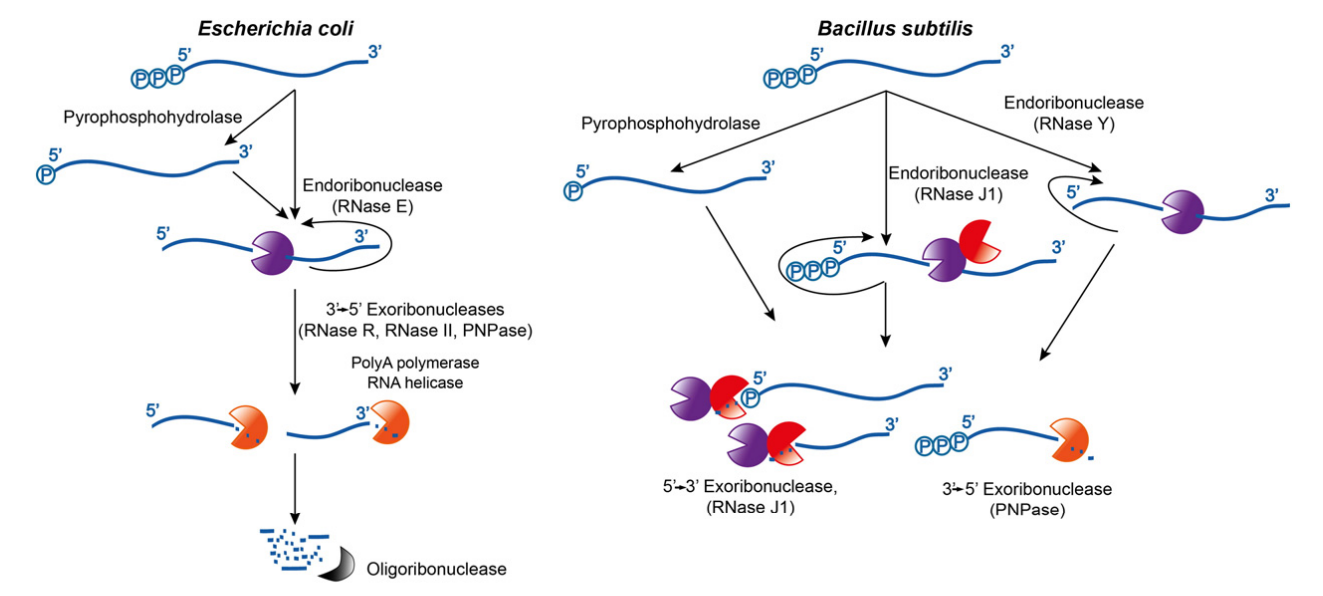
\includegraphics[width=0.9\linewidth]{figure/rnaDegradation}
	\caption{RNA degradation. Figure from \citet{bandyra_social_2013}.}
	\label{fig:rnaDegradation}
\end{figure}

RNA half-lives depend on the stability of the RNA, thus on its recognition by the degradosome or other ribonucleases. However, this stability is difficult to predict from the function of a gene, its sequence or even its secondary structure \citep{hambraeus_genome-wide_2003}. It is believed that ribosomes actively translating an mRNA protects it from being degraded by binding it, so that the RNA becomes unavailable for cleavage \citep{bandyra_licensing_2013}. Recent results shows that, while this is the case, it is not necessary to have ribosomes along the whole RNA, a ribosome can protect large parts of the mRNA "at distance" by making the docking of a specific part of the RNA impossible \citep{laalami_initiation_2013}. Whole genome studies yield distributions of RNA half-lives, showing that in \textit{B. subtilis}, most RNAs have a very short half-life (80\% shorter than 7 minutes) and a few have a relatively long half-life (3\% longer than 15 minutes) \citep{hambraeus_genome-wide_2003}. These half-lives probably vary depending on the physiological state of the cell. For example, targetting mRNAs with sRNAs is an efficient way to induce/inhibit translation (Fig. \ref{fig:srnaDegradation}).

\begin{figure}[!ht]
	\centering
	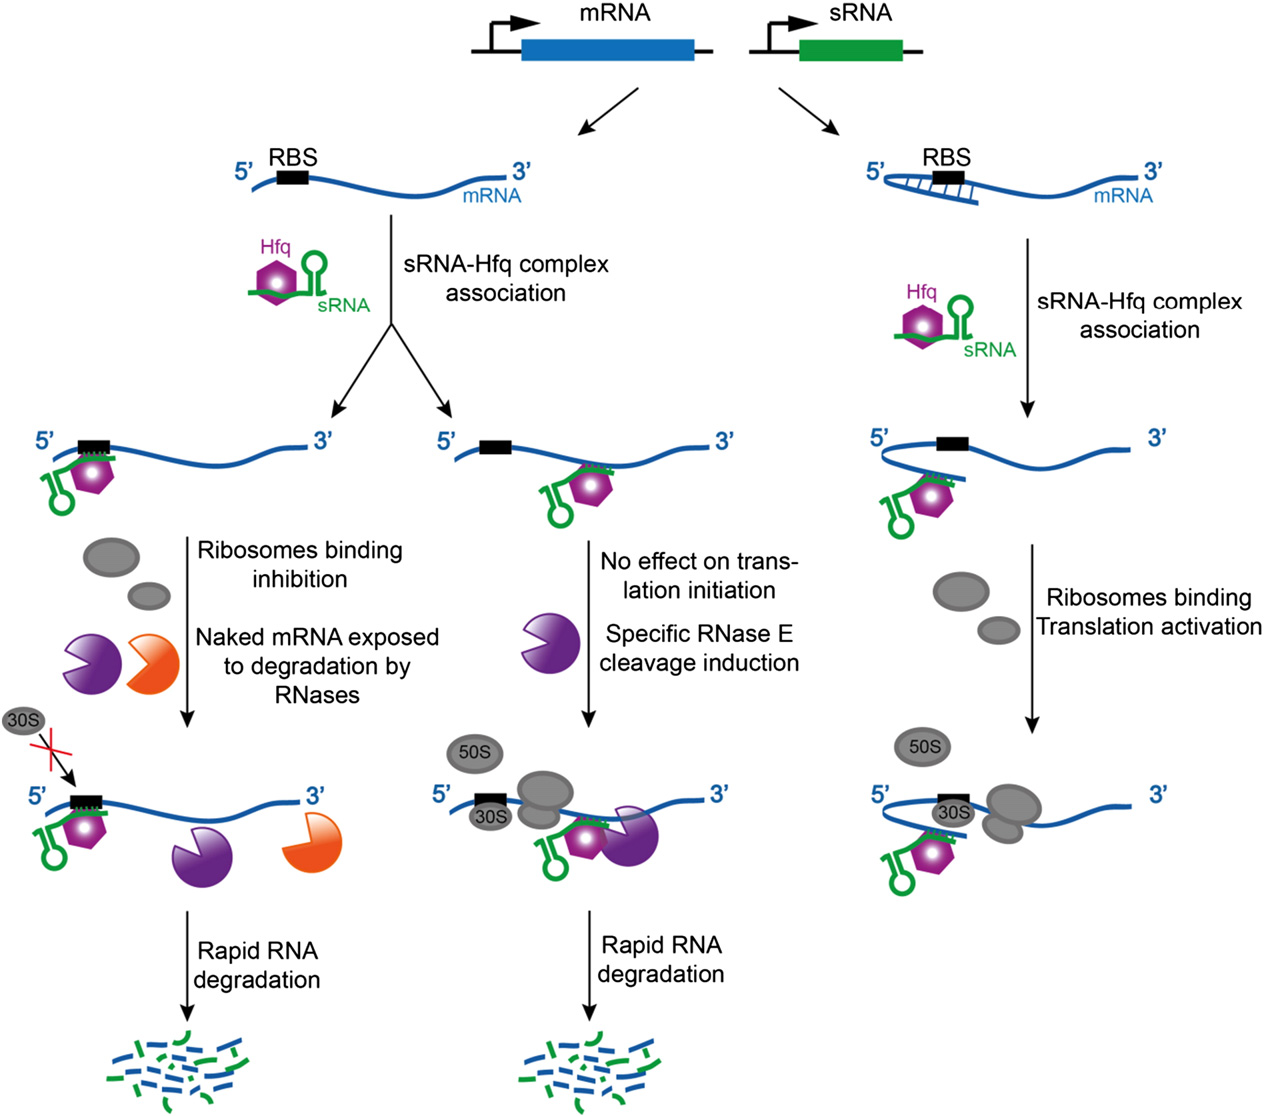
\includegraphics[width=0.9\linewidth]{figure/srnaDegradation}
	\caption{RNA control mediated by sRNAs. Figure from \citet{bandyra_social_2013}.}
	\label{fig:srnaDegradation}
\end{figure}

\subsection{Protein processes}

After being translated, a protein undergoes several processes before becoming mature. 5 important post-translational processes can be isolated (Figure \ref{fig:pTP}), even though they may occur in parallel. 3 processes are common to cytosolic, membrane and secreted proteins, namely
\begin{itemize}
\item Deformylation and demethylation.
\item Folding.
\item Residue modifications.
\end{itemize}

Moreover, there are 2 processes that specifically target membrane and secreted proteins
\begin{itemize}
\item Translocation.
\item Cleavage of the peptide signal and lipoprotein diacylglyceryl adduction.
\end{itemize}

\begin{figure}[!ht]
\centering
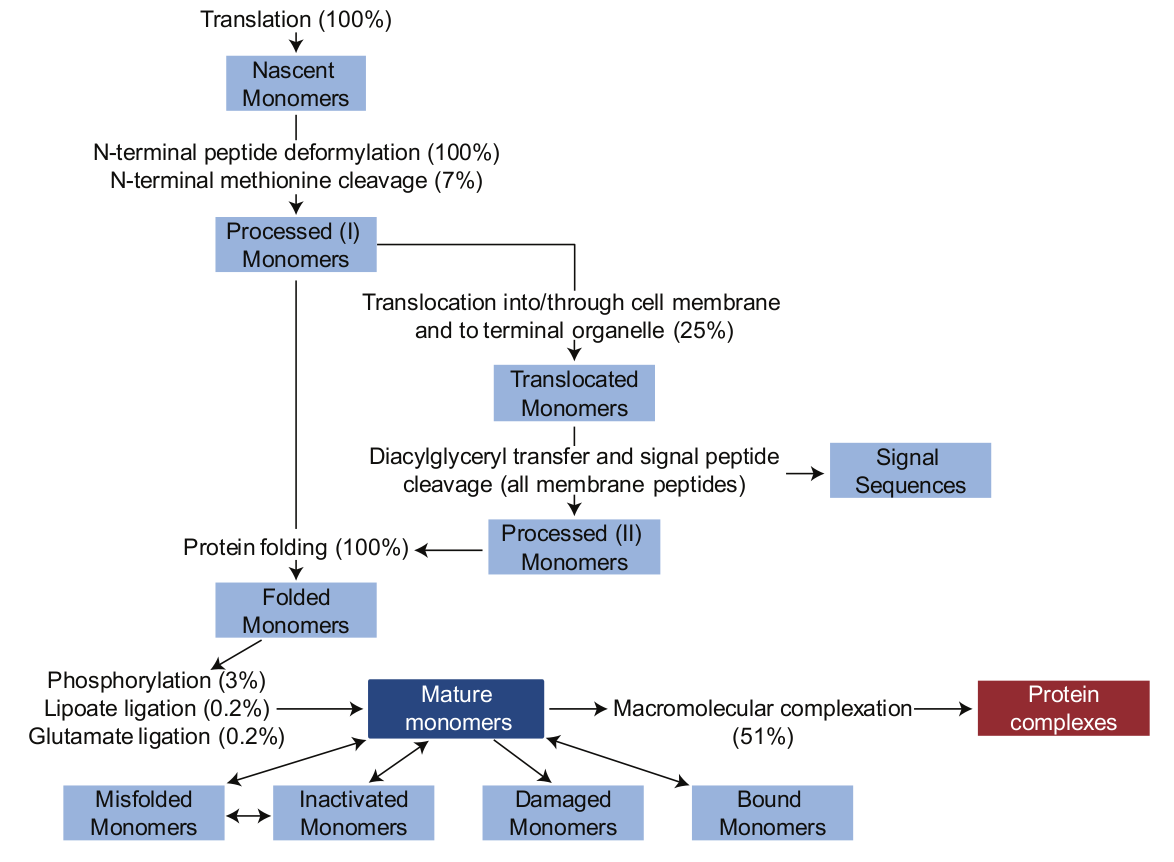
\includegraphics[width=0.8\linewidth]{figure/proteinProcesses}
\caption{Processes undergone by protein following translation (from Karr \textit{et al.})}
\label{fig:pTP}
\end{figure}

\subsubsection{Deformylation and demethylation}

For every protein, translation begins with a formylmethionine (fMet) residue. Several authors suggest that using exclusively fMet to start protein translation may be a way to regulate protein synthesis, as fMet is one of the most expensive amino acids to synthesize. Thus global protein synthesis levels would depend on global cell health.

This residue is then partially removed, but the role of deformylation and demethylation remains poorly understood. It may help in recycling fMet and influence protein degradation. According to the N-end rule, some N-terminal residues will lead to enhanced degradation. By changing the nature of the N-terminal residue, deformylation and demethylation allows for the N-end pathway to catalyze protein degradation.

Peptide deformylases (PDF) remove the formyl residue from fMet for most proteins. In \textit{B. subtilis}, YkrB is the main PDF, even though Def is known to have a similar action. It remains unclear whether these enzymes act during protein translation or after translation is completed. Methionine cleavage is performed by Methionine Aminopeptidases (MAP) but, contrarily to deformylation, it only targets a minority of proteins.

\subsubsection{Folding}

After translation, proteins can be viewed as a one-dimensional chain of amino acids. In order to acquire their functional form, proteins need to adopt a specific three-dimensional folding. Even though this folding is energetically favorable, numerous proteins need the help of another protein to adopt the proper conformation. These helper proteins are called chaperones. Bacteria use several chaperones. For example, in \textit{B. subtilis}
\begin{itemize}
\item The trigger factor Tig is known to assist early folding.
\item GroEL and its co-enzyme GroES assist late folding of short proteins.
\item DnaK, DnaJ and GrpE assist late folding of longer proteins.
\item FtsH may assist membrane protein folding.
\item Some proteins have specific chaperones (for example the translocated proteins TorA and NiFe are chaperoned by TorD and HybE respectively).
\end{itemize}

\subsubsection{Translocation, peptide signal cleavage and diacylglyceryl adduction}

During its life cycle, a bacterium heavily interacts with the extracellular medium. These interactions are enabled by proteins that are embedded in the membrane (nutrient transporters, ATP synthase, receptors, transducers) or secreted (virulence factors, cell wall components). Proteins that need to undergo translocation are identified by their N-terminal and C-terminal signal sequences (petide signals). Their embedding and secretion through the hydrophobic membrane is assisted by a specific machinery. 

Two important pathways are involved in protein translocation: Tat and SecA. They both involve a docking and a translocation step. Docking is mediated by peptide signals that can be recognized by signal recognition proteins (SRP) or directly by membrane proteins involved in the translocons (such as SecA or TatC). Translocation then occurs through a pore of variable size consisting of several proteins (SecYEG translocase or TatA like proteins). Depending on the nature of the proteins, translocation can occur simultaneously to translation (integral membrane proteins) or after translation (lipoproteins and secreted proteins). 

Following translocation, lipoproteins are anchored to the membrane through ligation of diacylglyceryl mediated by diacylglyceryl transferase and their peptide signal is removed by a signal peptidase. (what about the cleavage of peptide signals of secreted proteins and integral membrane proteins in \textit{B. subtilis} ???)


\subsubsection{Residue modifications}

Some proteins undergo post-translational chemical modifications. These modifications may serve different objectives such as favoring alternative conformations or regulating protein activity. Examples of residue modifications include phosphorylation, lipoyl transfer to lysine and $\alpha$-glutamate ligation, all catalyzed by specific enzymes.


\subsection{Stringent response}
\paragraph{Biological process} The stringent response is a fundamental regulation of the bacteria that regulates its growth rate and acts on practical all aspects of the cell. Discovered when amino-acid starving a bacteria (stringent response) compared to a rich nutriment response (relaxed response), the bacteria produces alarmones (p)ppGpp that induces the stringent response. Now stringent response means any response linked to the presence of the alarmones, including other stresses than the amino-acid starvation. The stringent response is different between {\it Escherichia Coli} and {\it Bacillus Subtilis} in its mechanism. The following text is principally based on the reviews of \citet{kriel_direct_2012} and of \citet{wolz_synthesis_2010}.

\medskip

{\bf Alarmones synthesis / hydrolysis}: Figure \ref{tab:compareColiSubAlarmoneProd} summarizes the current knowledge.
\begin{figure}[hbtp]
  \centering
  % Requires \usepackage{graphicx}
  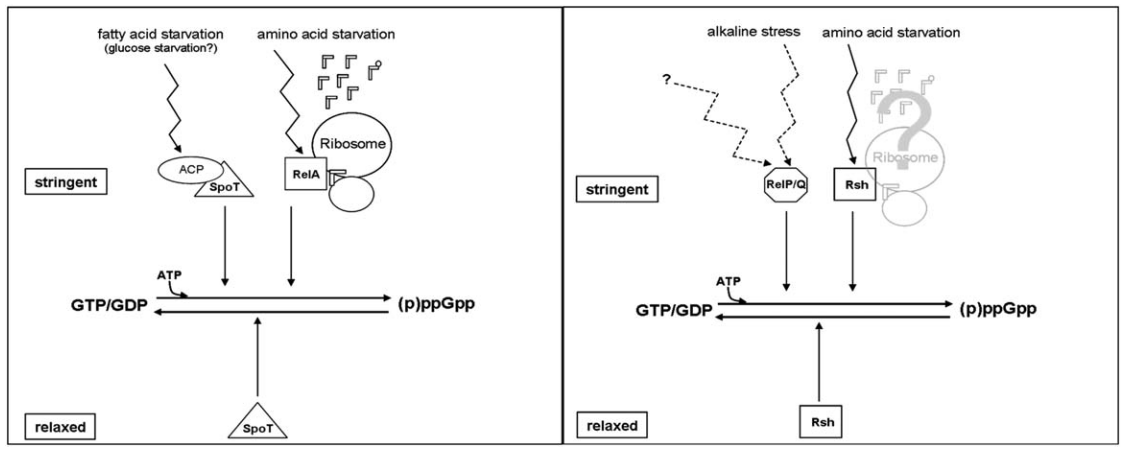
\includegraphics[width=15cm]{figure/alarmoneProd.png}\\
  \caption{Comparison of alarmones synthesis and hydrolysis between Escherichia Coli (left) and Bacillus Subtilis (right) \citep{wolz_synthesis_2010}}\label{tab:compareColiSubAlarmoneProd}
\end{figure}
Rsh (which is also referred to as RelA) in {\it B. Subtilis} and SpoT in {\it E. Coli} are bifunctional (the others being monofunctional) enzymes that can perform synthesis and hydrolysis. They have two conformations ((p)ppGpp-hydrolase-OFF/(p)ppGpp-synthase-ON and hydrolase-ON/synthase-OFF) that is regulated by the C-terminal domain as its truncation enhances the synthase activity. It is not known if, as in the case of {\it E. Coli}, Rsh binds to a ribosome to sense the amino-acid starvation and more precisely the presence of uncharged tRNA. In {\it E. Coli}, RelA binds to a ribosome and is thought to unbind in the presence of an uncharged tRNA in the A-site. This unbinding activates the synthetase function of RelA and inhibits the rebinding during a period of time. In {\it B. Subtilis}, it is knwon that there are only one bifunctional enzyme (Rsh) and only two monofunctional ones (RelP seems to be connected to competence and is encoded by yjbM whereas RelQ seems to be connected to persistence and virulence and is encoded by ywaC) that lack the \ce{Mn^2+}-dependent hydrolase domain \citep{GaL:15}.

\medskip

{\bf Overall effect of alarmones}: it is estimated that, in exponential gorwth conditions, the concentration of alarmones is less than 20 pmol per optical-density unit by rises to millimolar levels in response to adverse growth conditions, such as amino acid starvation \citep{ababneh_rela_2015}. The effect of the alarmones on proteobacteria ({\it E. Coli}) and firmicutes ({\it B. Subitlis}) is summarized in Table \ref{tab:compareColiSubPhysiology}. Alarmones affects the majors process of the bacteria: replication, transcription and translation. The means are however different.
\begin{table}[hbtp]
  \centering
  % Requires \usepackage{graphicx}
  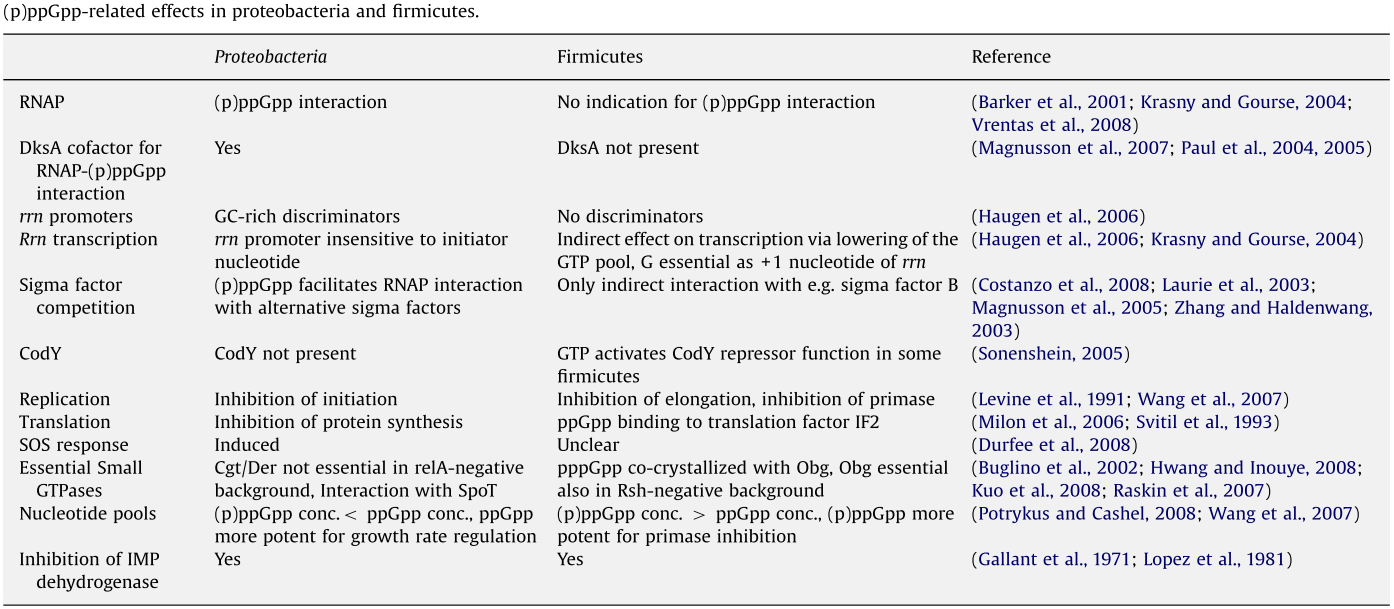
\includegraphics[width=17cm]{figure/compareStringentColiSubtilisTable.png}\\
  \caption{Comparison of stringent response between Escherichia Coli and Bacillus Subtilis \citep{wolz_synthesis_2010}}\label{tab:compareColiSubPhysiology}
\end{table}
More generally, it is suggested in \citep{kanjee_direct_2012} that the alarmones can bind in place of GTP in the three GTPase categories: translation elongation (EF-G, EF-Tu, IF2), cell-signalling and cell-division (Obg) and protein translocation.

\medskip

{\bf Alarmones effect on GTP concentration}: in {\it B. Subtilis}, the alarmones regulates the pool of ATP and GTP as shown in Figure \ref{fig:alarmoneEnergyReg}.
\begin{figure}[hbtp]
  \centering
  % Requires \usepackage{graphicx}
  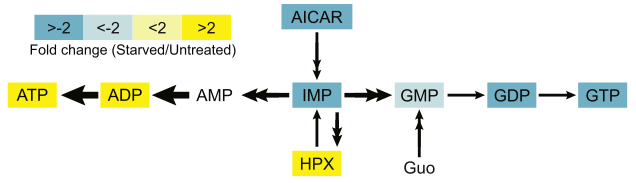
\includegraphics[width=15cm]{figure/alarmoneEnergy.png}\\
  \caption{Bacillus Subtilis: regulation of ATP and GTP pool by the alarmones \citep{kriel_direct_2012}}\label{fig:alarmoneEnergyReg}
\end{figure}
This is illustrated in more details in Figure \ref{fig:alarmoneGTPReg}.
\begin{figure}[hbtp]
  \centering
  % Requires \usepackage{graphicx}
  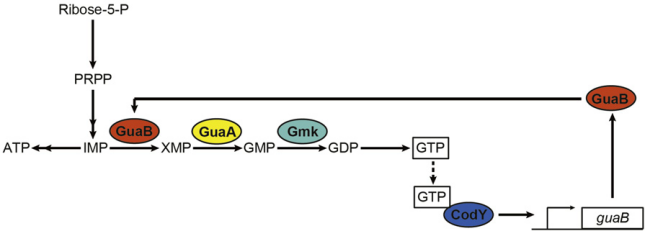
\includegraphics[width=10cm]{figure/alarmoneGTPPathway1.png} \\ 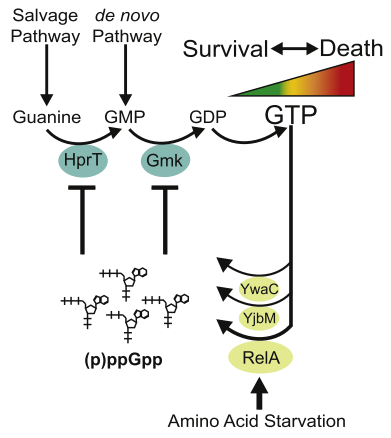
\includegraphics[width=6cm]{figure/alarmoneGTPPathway2.png}\\
  \caption{Bacillus Subtilis: GTP pathway regulation \citep{kriel_direct_2012}}\label{fig:alarmoneGTPReg}
\end{figure}
The regulation of GTP pool via the alarmones is more importantly performed by Gmk and HprT than by GuaB \citep{kriel_direct_2012}. The $IC_{50}$ are: $\approx 20 \mu M$ for Gmk, $\approx 11 \mu M$ for HprT and $\approx 0.3-0.5 mM$ for GuaB.





\subsection{Metabolism}
\textcolor[rgb]{1.00,0.00,0.00}{\textbf{\emph{\huge Joker!}}}

\subsection{Volume growth}
\textcolor[rgb]{1.00,0.00,0.00}{When? Where?}

\subsection{Exchanges}
\subsubsection{Exchange with extracellular conditions}
Not described but a matter of changing the pool (concentrations probably for extracellular conditions) in volume and extracellular conditions. Works in both ways if needed.

\subsubsection{Exchange between volumes}
\textcolor[rgb]{1.00,0.00,0.00}{Not described but a matter of changing the pool in volumes. Works in both ways if needed. Just remind that for 'complex' entities, it is easier if everything is contained in one entity only. I mean, if a mRNA binded with a 70S and an AA 1 charged tRNA moves, then if only one entity contains all these information, it is much easier. Here we would have chosen the mRNA.} 

\subsection{Volume division}
\textcolor[rgb]{1.00,0.00,0.00}{Need to obtain a storage for interface between volume. But otherwise, volume division is a matter of deleting a volume, creating 2 (3? 4?) volumes, adjusting the interfaces and pools. Needs to be a cell process since it can change the chromosome location.} 

\subsection{Cytokinesis, cell fission?}

\begin{figure}[!ht]
	\centering
	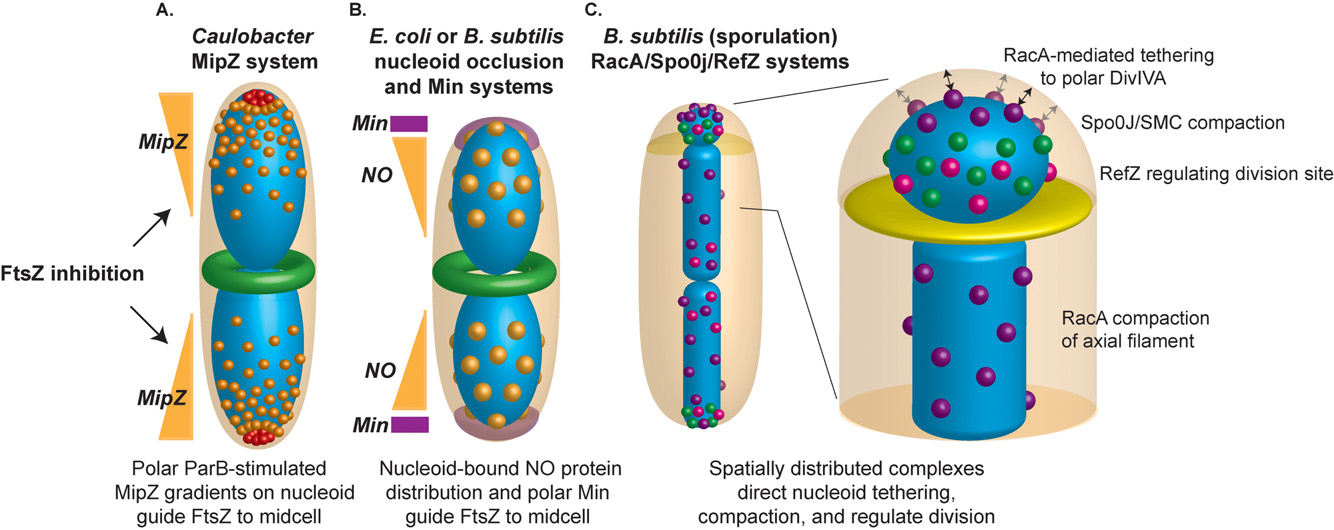
\includegraphics[width=0.9\linewidth]{figure/cytokinesis}
	\caption{Figure from \citet{ptacin_chromosome_2013}}
	\label{fig:cytokinesis}
\end{figure}

\textcolor[rgb]{1.00,0.00,0.00}{Depending on how it is modeled. The part on geometry is 'simple' to model:
\begin{itemize}
  \item volume division;
  \item changing the characteristics of the concerned volumes to adjust the surface of exchange for example.
\end{itemize}
Other part? Needs to be a cell process.}

\subsection{Processes from wholeCell}
Police barr\'{e}e = un process de wholeCell que j'ai remis en haut, sans pour autant l'avoir mod\'{e}liser ou avoir les informations n\'{e}cessaires dans les \'{e}tats.
\begin{itemize}
  \item \sout{Chromosome condensation: DNA clamping by SMC complexes}
  \item \sout{Chromosome segregation}
  \item \sout{Cytokinesis: pinching of the cell membrane}
  \item \sout{DNA damage: Gap site, Abasic site, Sugar-phosphate, Base, Intrastrand cross link, Strand break, Holliday junction}
  \item \sout{DNA repair}
  \item \sout{DNA supercoiling}
  \item FtsZ polymerization
  \item Host interaction: des trucs mais en quoi c'est utile ?
  \item Macromolecular complexation: models the formation of all macromolecular complexes except the 30S and 50S ribosomal particles, the 70S ribosome, the FtsZ ring, and the oriC DnaA complex
  \item \sout{Metabolism: models the import of extracellular nutrients and their conversion into macromolecule building blocks}
  \item Protein activation:  implements a Boolean model of their effects on the functional state – enzymatically competent or incompetent – of mature proteins
  \item Protein decay: models the degradation of protein monomers, macromolecular complexes, cleaved signal sequences, and prematurely aborted polypeptides as well as the misfolding and refolding of protein monomers and complexes
  \item Protein folding
  \item Protein modification: models protein covalent modification including phosphorylation, lipoyl transfer, and α-glutamate ligation
  \item Protein processing I: models N-terminal formylmethionine deformylation and N-terminal methionine cleavage, the first steps in post-translational processing. What's that???
  \item Protein processing II: models the third step of post-translational processing: lipoprotein diacylglyceryl adduction and lipoprotein and secreted protein signal peptide cleavage. What's that?
  \item Protein translocation: models membrane and extracellular protein localization, the second step in post-translational processing
  \item \sout{Replication}
  \item Replication initialization: determines when during the cell cycle chromosome duplication begins. Uses the protein DnaA (MG469)
  \item \sout{Ribosome assembly:  models the enzyme-catalyzed formation of 30S and 50S ribosomal particles}
  \item RNA decay: decays all species of RNA, and at all maturation states including aminoacylated states
  \item RNA modification: the exact role of rRNA modification is unknown. This process models tRNA and rRNA modification
  \item RNA processing:  models operonic RNA cleavage into individual RNA gene products. Something about operons.
  \item Terminal organelle assembly: models the assembly of the protein content of the terminal organelle
  \item \sout{Transcription: For simplicity, our model doesn’t represent this phenomenon, allowing translation only of completed mRNAs}
  \item Transcription regulation: models the binding of transcriptional regulators to promoters and the fold-change effect of transcriptional regulators on the affinity of RNA polymerase for individual promoters.
  \item \sout{Translation}
  \item \sout{tRNA aminocylation}
\end{itemize}


\end{document}
% ----------------------------------------------------------------
